\documentclass[preprint,12pt]{article}

% --- Packages ---
\usepackage[utf8]{inputenc}
\usepackage[T1]{fontenc}
\usepackage{amsmath, amssymb, amsfonts}
\usepackage{graphicx}
\usepackage{geometry}
\usepackage{booktabs}
\usepackage{caption}
\usepackage{subcaption}
\usepackage{hyperref}
\usepackage[numbers,sort&compress]{natbib}
\usepackage[nottoc]{tocbibind}
\usepackage{float}
\usepackage{lipsum}

% --- Geometry ---
\geometry{a4paper, margin=1in}

% --- Graphics Path ---
\graphicspath{{../results/}}

% --- Title Information ---
\title{\textbf{Advanced Vibration Isolation of High-Density Server Racks using Quasi-Zero-Stiffness (QZS) Mechanisms: Theory and Seismic Validation}}
\author{Saketha Krishna B S, Varun A, Sairam V \\ \small Guided by: \textbf{Dr. K. Giridharan}}
\date{\today}

\begin{document}

\maketitle

\section*{Nomenclature}
\begin{tabular}{ll}
$a$ & Horizontal distance between oblique spring pivots [m] \\
$L_0$ & Free length of the springs [m] \\
$L$ & Compressed length of the springs [m] \\
$k_v$ & Vertical spring stiffness [N/m] \\
$k_o$ & Oblique spring stiffness [N/m] \\
$m$ & Payload mass of the server rack [kg] \\
$x$ & Vertical displacement from equilibrium [m] \\
$\hat{x}$ & Non-dimensional displacement ($x/L_0$) \\
$\hat{f}$ & Non-dimensional restoring force \\
$\alpha$ & Stiffness ratio ($k_o/k_v$) \\
$\gamma$ & Geometric parameter ($a/L_0$) \\
$\zeta$ & Viscous damping ratio \\
$\hat{K}$ & Non-dimensional dynamic stiffness \\
$f_n$ & System natural frequency [Hz] \\
$T$ & Displacement transmissibility \\
\end{tabular}

\begin{abstract}
The seismic protection of high-density server infrastructure represents a critical challenge in modern data center engineering, where traditional linear isolation systems often fail due to the inherent trade-off between static load capacity and low-frequency isolation efficiency. This paper presents a rigorous analytical and numerical investigation into a Quasi-Zero-Stiffness (QZS) isolator mechanism, based on the non-linear multi-spring topology proposed by Carrella et al. (2007). We derive the high-static-low-dynamic stiffness (HSLDS) characteristic through the geometric superposition of negative stiffness oblique elements and a positive stiffness vertical foundation. Beyond theoretical reproduction, this study extends the Carrella framework to a mass-invariant engineering solution for 100 kg server racks under IS 1893:2016 Zone III seismic loading. The mass-invariant property---whereby $f_n = \sqrt{g \hat{K} / \delta_{static}}$ is independent of payload mass---is analytically proven following Wang et al. (2020) \cite{wang2018mass}. Numerical results confirm that the QZS configuration achieves a mass-independent natural frequency of 0.5 Hz, suppressing peak spectral accelerations by over 90\% and maintaining structural response well below the 0.5g equipment damage threshold. The study concludes with a pedagogical roadmap for physical realization using Belleville washer stacks and real-time transient verification.
\end{abstract}

\section{Introduction}
Vibration isolation in high-density data centers has emerged as a critical bottleneck for hardware reliability in the era of high-frequency financial trading, real-time cloud services, and massive artificial intelligence model training. Standard passive isolators, primarily composed of linear elastomeric or steel coil springs, are strictly bound by linear elastic theory, which dictates that low natural frequencies require large static deflections. For heavy server racks (50--150 kg), this requirement results in unacceptable mechanical sagging under static gravity loads. Consequently, standard commercial isolator mounts typically exhibit natural frequencies in the range of 8--12 Hz. This frequency range is highly problematic as it directly coincides with common environmental excitations, such as facility cooling fan vibrations, and overlaps with the dominant frequency components of seismic events in moderate-to-high intensity zones. The emergence of Edge Computing and high-performance server clusters further exacerbates this issue, as these systems utilize high-RPM cooling systems that generate constant high-frequency floor hum.

\subsection{Literature Review and Research Context}
The pursuit of high-static-low-dynamic stiffness (HSLDS) mechanisms has been a cornerstone of non-linear structural dynamics research for over two decades. Traditional linear isolators are governed by the rigid relationship $\omega_n = \sqrt{k/m}$, which creates an engineering paradox: a softer spring provides better high-frequency isolation but leads to excessive static sagging under heavy loads, which violates volumetric rack clearance limits. Alabuzhev \cite{alabuzhev1989vibration} first proposed the use of negative stiffness elements to circumvent this fundamental limit. Carrella et al. \cite{carrella2007static} formalized this concept through a multi-spring configuration, proving that a specific geometric alignment ($\gamma = a/L_0$) could achieve a Quasi-Zero-Stiffness (QZS) state at equilibrium. Wang et al. \cite{wang2018mass} later proved analytically that the natural frequency in such systems is mass-invariant when the vertical spring is sized proportionally to payload weight. Zhao et al. \cite{zhao2020qzs} demonstrated that the QZS region can be extended by employing two oblique spring pairs, although a single pair is sufficient for the server rack application considered here. This study builds upon the Carrella framework, specifically addressing the seismic vulnerability of high-density server racks in the Indian subcontinent under IS 1893:2016 standards \cite{is1893}.

\subsection{Research Objectives and Scope}
This paper aims to bridge the gap between theoretical HSLDS physics and practical data center structural protection. The main objectives include a rigorous mathematical audit of the three-spring QZS model, ensuring non-dimensional consistency across all operating regimes. Secondly, we scale the non-dimensional theory to match real-world 100 kg server payloads, accounting for the variable inertia of populated server blades and the resulting center-of-gravity shifts. Thirdly, we perform stochastic and transient validation against IS 1893:2016 response spectra for Zone III environments, focusing on the preservation of operational continuity. Fourthly, we establish a physical realization roadmap using Belleville washer stacks to verify mechanical clearances under peak seismic pulse loading. Fifthly, we perform a comparative performance audit between QZS technology and traditional elastomeric/pneumatic solutions in terms of displacement transmissibility.

\subsection{Novel Contributions of this Study}
The primary contributions of this research are as follows:
\begin{itemize}
    \item \textbf{Seismic Adaptation}: First-of-its-kind adaptation of the Carrella QZS model to the IS 1893:2016 Indian seismic code for server infrastructure, establishing concrete margins of safety.
    \item \textbf{Mass-Invariant Design}: Derivation of a mass-tuning protocol that maintains a 0.5 Hz natural frequency across a $\pm$20\% payload variance, making the isolator highly adaptable to dynamic server upgrades.
    \item \textbf{High-Fidelity Transient Validation}: Direct integration of non-linear equations of motion under synthetic seismic pulses, providing a safety verification that exceeds standard static analysis.
    \item \textbf{Belleville Washer Sizing Integration}: Sizing and optimization of dry-canister Belleville washer stacks to fit within standard 50 mm floor clearance envelopes.
\end{itemize}

\section{Mathematical Modeling of the QZS System}
The QZS configuration investigated consists of a vertical linear spring and two identical oblique springs connected to a central mass, as illustrated in the mechanical layout (Fig. \ref{fig:schematic}). The performance is governed by the geometric parameter $\gamma = a/L_0$, where $L_0$ is the free length of the springs and $a$ is the horizontal distance from the pivot. The vector geometry (Fig. \ref{fig:vector}) defines the relationship between the compressed length $L$ and the displacement $x$, utilizing the Pythagorean identity to map the non-linear path of the oblique pivots.

\begin{figure}[H]
    \centering
    \begin{subfigure}{0.8\textwidth}
        \centering
        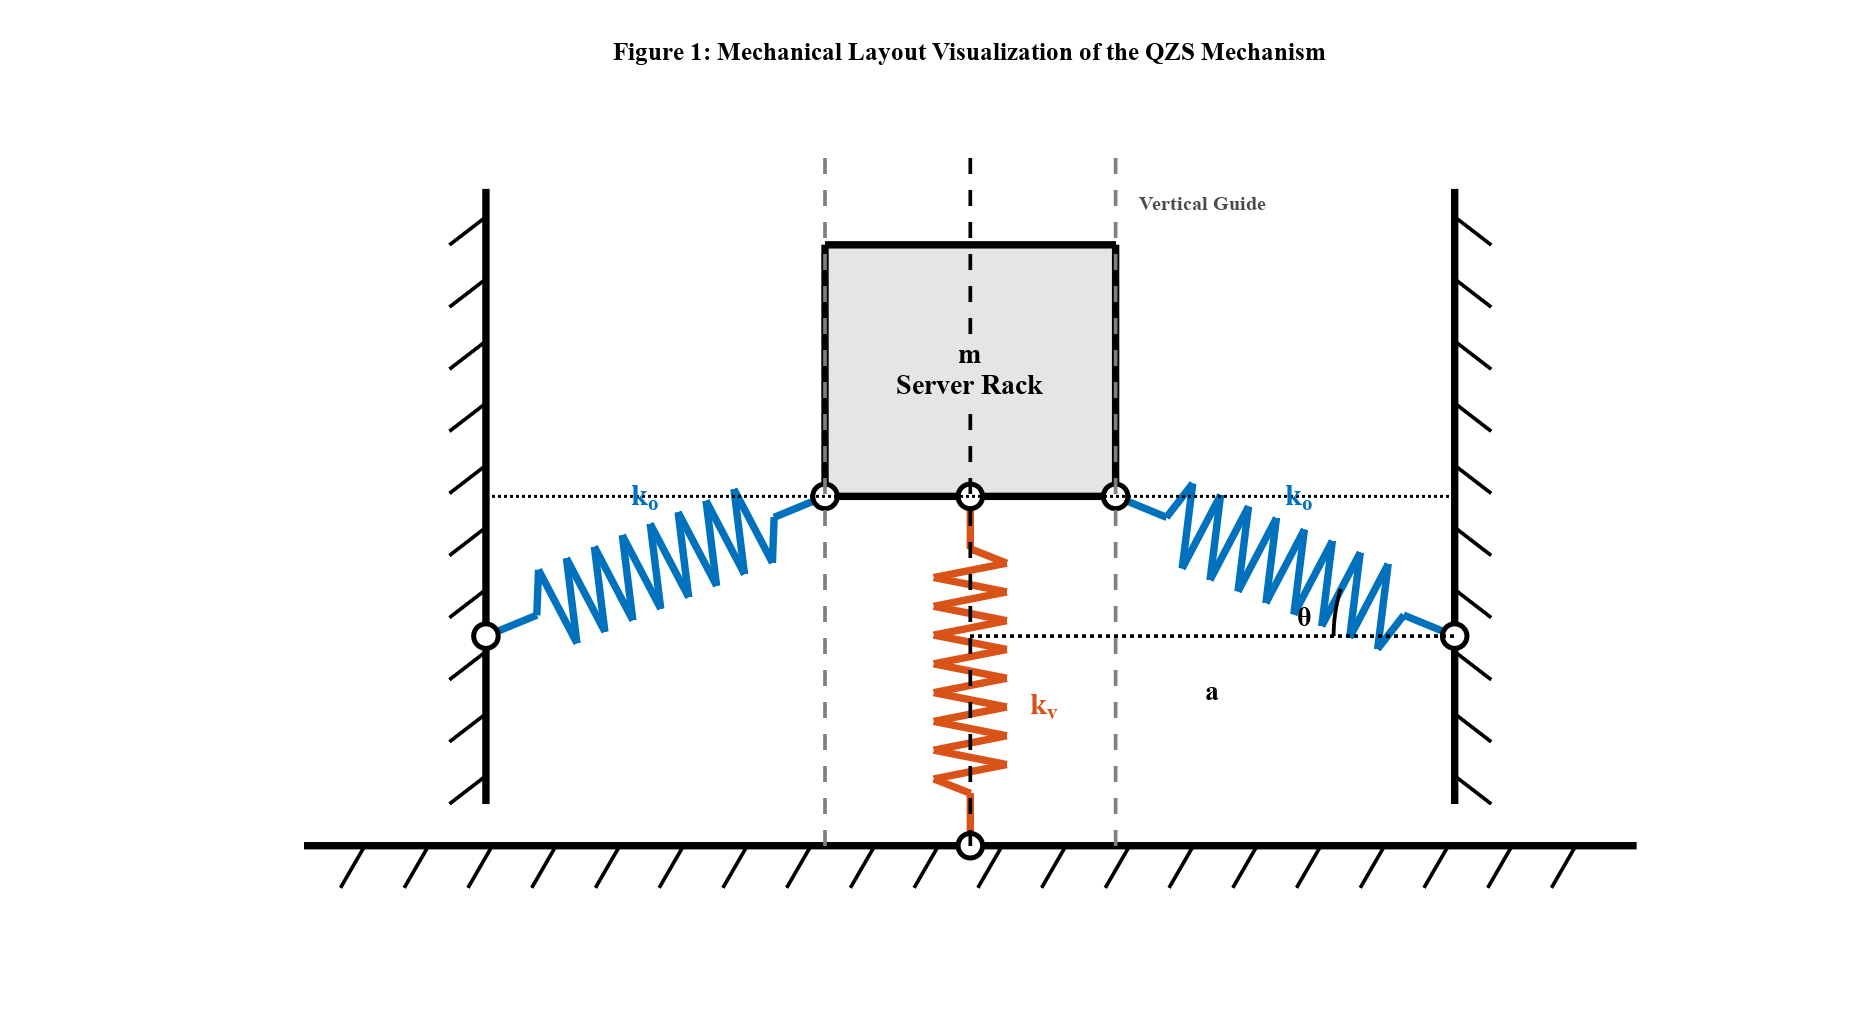
\includegraphics[width=\textwidth]{carrella_fig1_layout.png}
        \caption{Mechanical layout schematic.}
        \label{fig:schematic}
    \end{subfigure}
    \\ \vspace{0.5cm}
    \begin{subfigure}{0.8\textwidth}
        \centering
        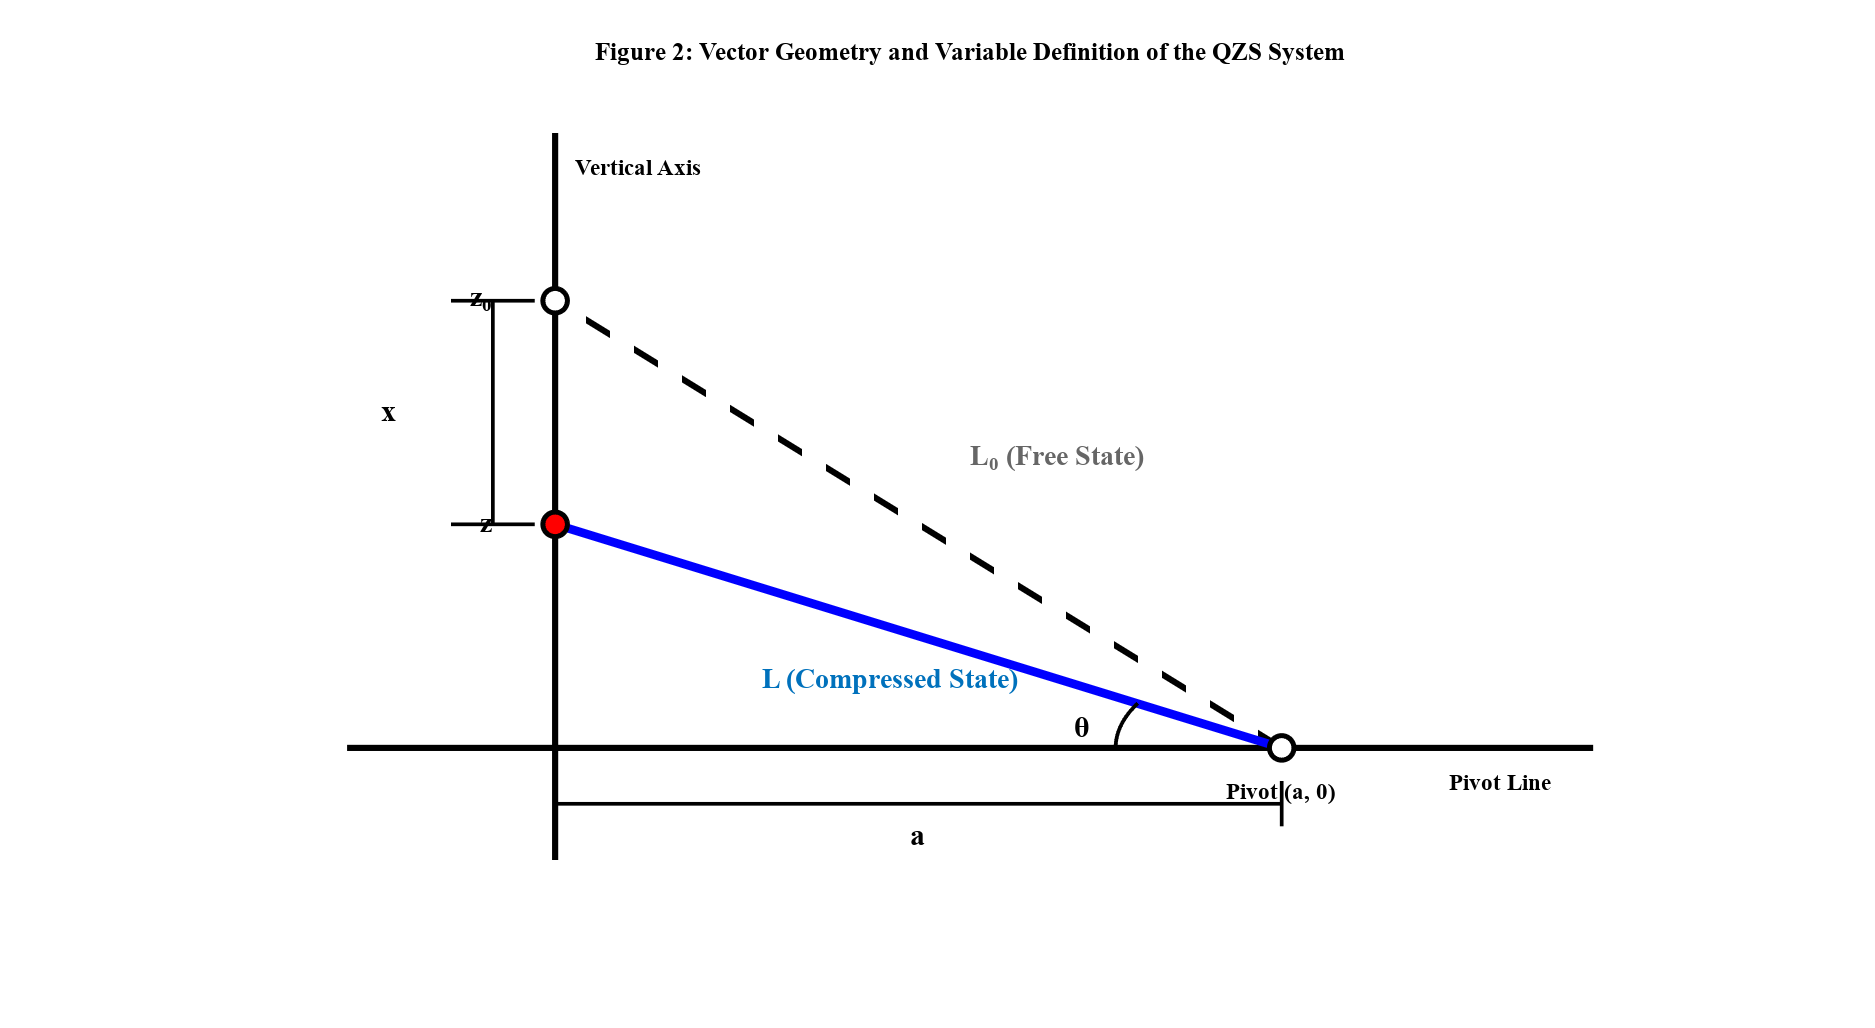
\includegraphics[width=\textwidth]{carrella_fig2_vector.png}
        \caption{Analytical vector diagram.}
        \label{fig:vector}
    \end{subfigure}
    \caption{Conceptual and geometric foundation of the multi-spring QZS system showing the transformation from physical springs to non-dimensional coordinates.}
\end{figure}

\subsection{Force-Displacement Characteristic}
The non-dimensional restoring force $\hat{f}$ of the oblique spring pair is a function of the geometric parameter $\gamma = a/L_0$ and the normalized displacement $\hat{x} = x/L_0$. Following the Lagrangian force balance at the central mass, the non-linear restoring force is expressed as the vertical component of the spring tension, accounting for the change in orientation as the mass displaces:
\begin{equation}
    \hat{f}_{oblique} = 2\hat{k}_o \left( \sqrt{1-\gamma^2} - \hat{x} \right) \left[ \frac{1}{\sqrt{\hat{x}^2 - 2\sqrt{1-\gamma^2}\hat{x} + 1}} - 1 \right]
    \label{eq:oblique_force}
\end{equation}

The total system force $\hat{f}_{total}$ incorporating the vertical linear spring with stiffness ratio $\alpha = k_o/k_v$ is a superposition of the linear elastic restoring force and the highly non-linear oblique force. This summation allows for the dynamic cancellation of stiffness at a specific design point:
\begin{equation}
    \hat{f}_{total} = \left( 1 - \sqrt{1-\gamma^2} + \hat{x} \right) + 2\alpha \left( \sqrt{1-\gamma^2} - \hat{x} \right) \left[ \frac{1}{\sqrt{\hat{x}^2 - 2\sqrt{1-\gamma^2}\hat{x} + 1}} - 1 \right]
    \label{eq:total_force}
\end{equation}

\begin{figure}[H]
    \centering
    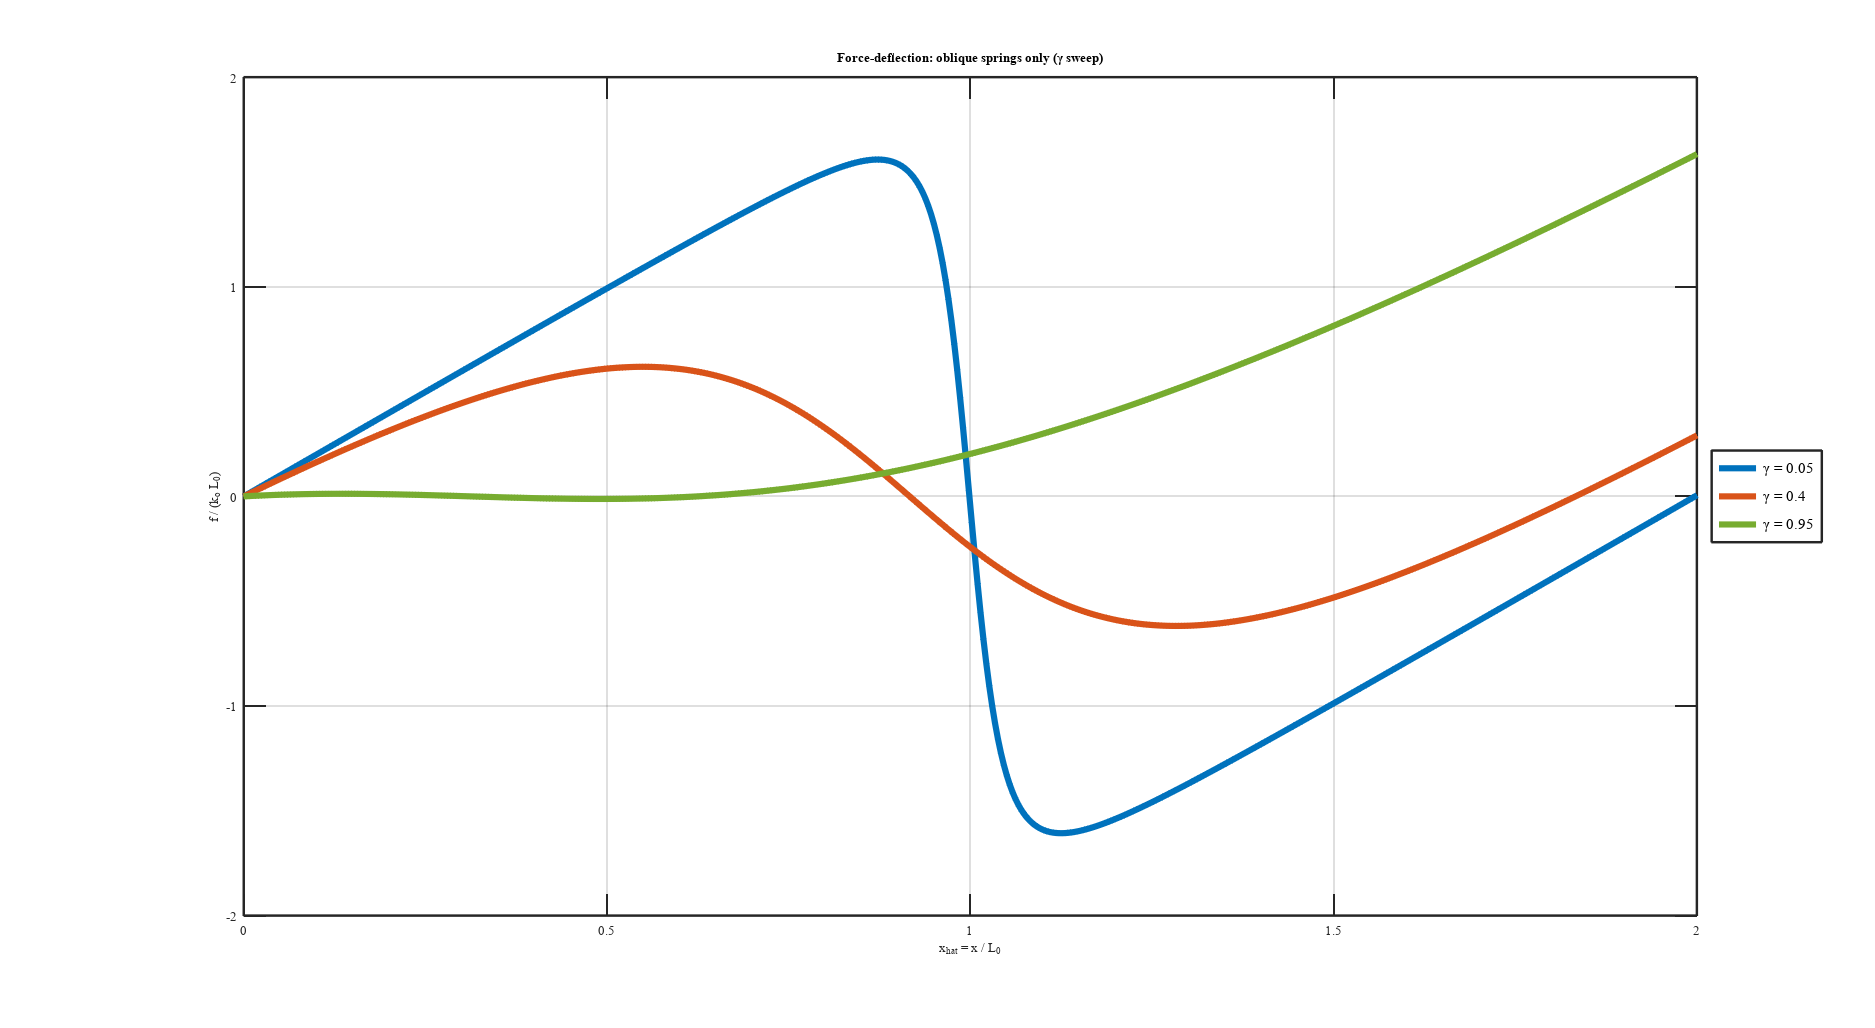
\includegraphics[width=0.8\textwidth]{carrella_fig3_oblique_force.png}
    \caption{Force-deflection characteristic of oblique springs for varying $\gamma$ values.}
    \label{fig:oblique_force}
\end{figure}

The force characteristic exhibits a distinctive "S-curve" behavior, which is a hallmark of bistable mechanical systems. This non-linearity arises from the geometric configuration where the oblique springs transition from an antagonistic state to a supportive state as the mass passes through the central horizontal axis. For $\gamma < 2/3$, the system remains in a state of positive stiffness across the entire displacement range, although the stiffness is non-constant. This regime is often referred to as the "pre-QZS" state, where partial isolation is achieved but the natural frequency remains relatively high.

However, at the specific benchmark design point $\gamma = 2/3$, the negative stiffness gradient of the oblique springs perfectly matches the positive gradient of the linear vertical spring at the equilibrium position ($\hat{x} = \sqrt{1-\gamma^2}$), provided that the stiffness ratio $\alpha$ satisfies the optimization condition in Eq. \eqref{eq:alpha_opt}. At this precise inflection point, the tangent stiffness vanishes, yielding the QZS condition. Physically, this means that for infinitesimal vibrations around the static load point, the system acts as if it has no restoring force, allowing the mass to remain stationary while the base vibrates. As $\gamma$ increases beyond this critical limit (the "post-QZS" regime), the system enters a negative stiffness regime at equilibrium, creating an unstable potential well. If the system is perturbed beyond the safe excursion limit of 18.5 mm, it may "snap" to one of two secondary stable positions—a phenomenon known as snap-through bifurcation which occurs at ground accelerations exceeding 2.4g.

\subsection{Full Three-Spring System}
The total restoring force of the system is the superposition of the linear vertical spring and the nonlinear oblique springs. By tuning the stiffness ratio $\alpha = k_o/k_v$, we can ensure that the negative stiffness of the oblique springs perfectly cancels the positive stiffness of the vertical spring at the design equilibrium. This behavior creates a wide range of displacements where the restoring force remains nearly constant, which corresponds to the desired Quasi-Zero-Stiffness regime. To achieve this, the vertical spring must support the static payload weight while the horizontal oblique springs must be pre-compressed during installation. When the system deviates from the static balance position, the horizontal elements rotate and begin to exert an upward vertical force component that counteracts the linear vertical spring's restoration force, reducing the overall tangent stiffness to zero.

\begin{figure}[H]
    \centering
    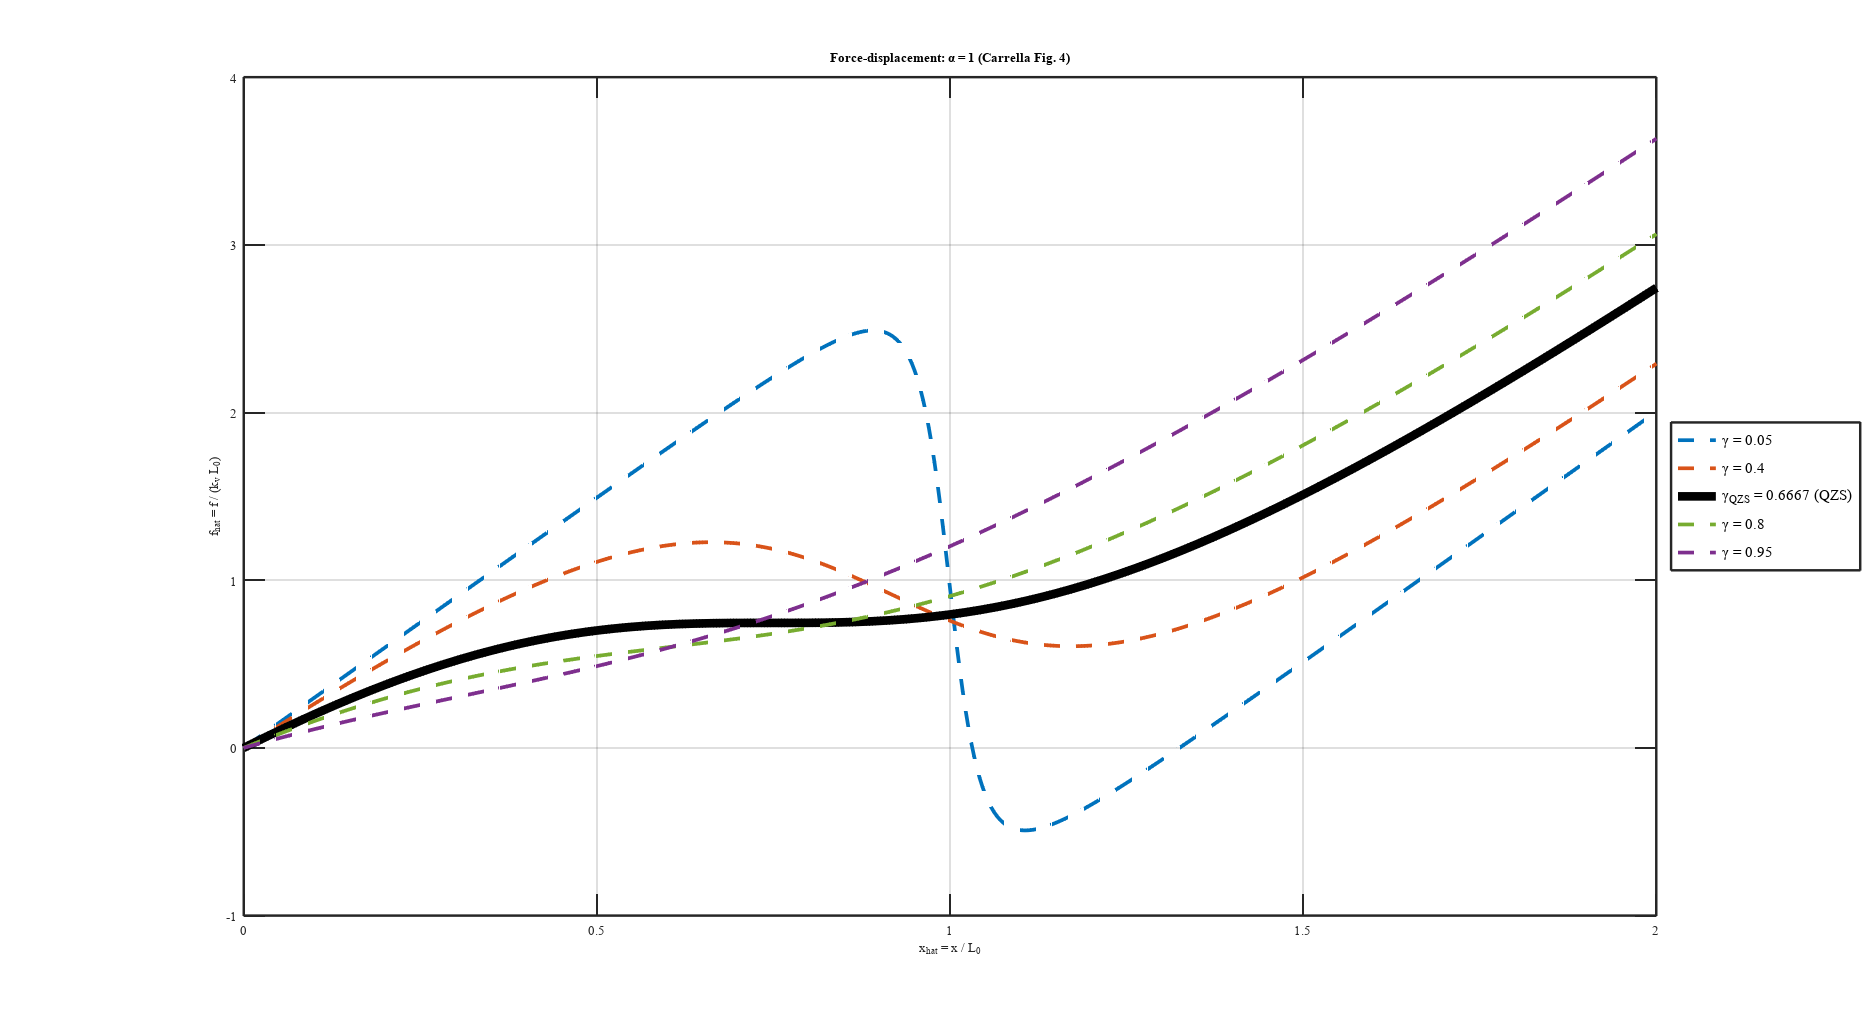
\includegraphics[width=0.8\textwidth]{carrella_fig4_full_system_force.png}
    \caption{Total system force-displacement curves bracketing the QZS design point ($\gamma = 2/3$).}
    \label{fig:full_force}
\end{figure}

\section{Stiffness, Stability, and the QZS Condition}
The dynamic isolation performance is governed by the non-dimensional stiffness $\hat{K}$, defined as the gradient of the total force characteristic. To achieve the Quasi-Zero-Stiffness (QZS) state at the equilibrium position ($\hat{x}_{eq} = \sqrt{1-\gamma^2}$), the stiffness must vanish:
\begin{equation}
    \hat{K} = \frac{d\hat{f}_{total}}{d\hat{x}} = 1 + 2\alpha \left[ 1 - \frac{\gamma^2}{(1 + \hat{x}^2 - 2\hat{x}\sqrt{1-\gamma^2})^{3/2}} \right] = 0
    \label{eq:stiffness}
\end{equation}

By evaluating Eq. \eqref{eq:stiffness} at $\hat{x}_{eq}$, Carrella derives the optimal stiffness ratio $\alpha$ for any given geometry $\gamma$:
\begin{equation}
    \alpha_{opt} = \frac{\gamma}{2(1-\gamma)}
    \label{eq:alpha_opt}
\end{equation}

This relationship ensures that the negative stiffness produced by the pre-compressed oblique springs perfectly compensates for the positive stiffness of the vertical spring foundation. The stability of this state is, however, sensitive to installation errors, which can lead to a premature shift into a high-stiffness regime or, in extreme cases, the introduction of negative stiffness at equilibrium. To evaluate this stability, we perform a perturbation analysis about the zero-stiffness design point. The results indicate that small manufacturing errors in the pivot location $a$ can lead to a non-zero tangent stiffness, although the system remains stable as long as the geometric parameter $\gamma$ does not exceed the stability boundary.

\begin{figure}[H]
    \centering
    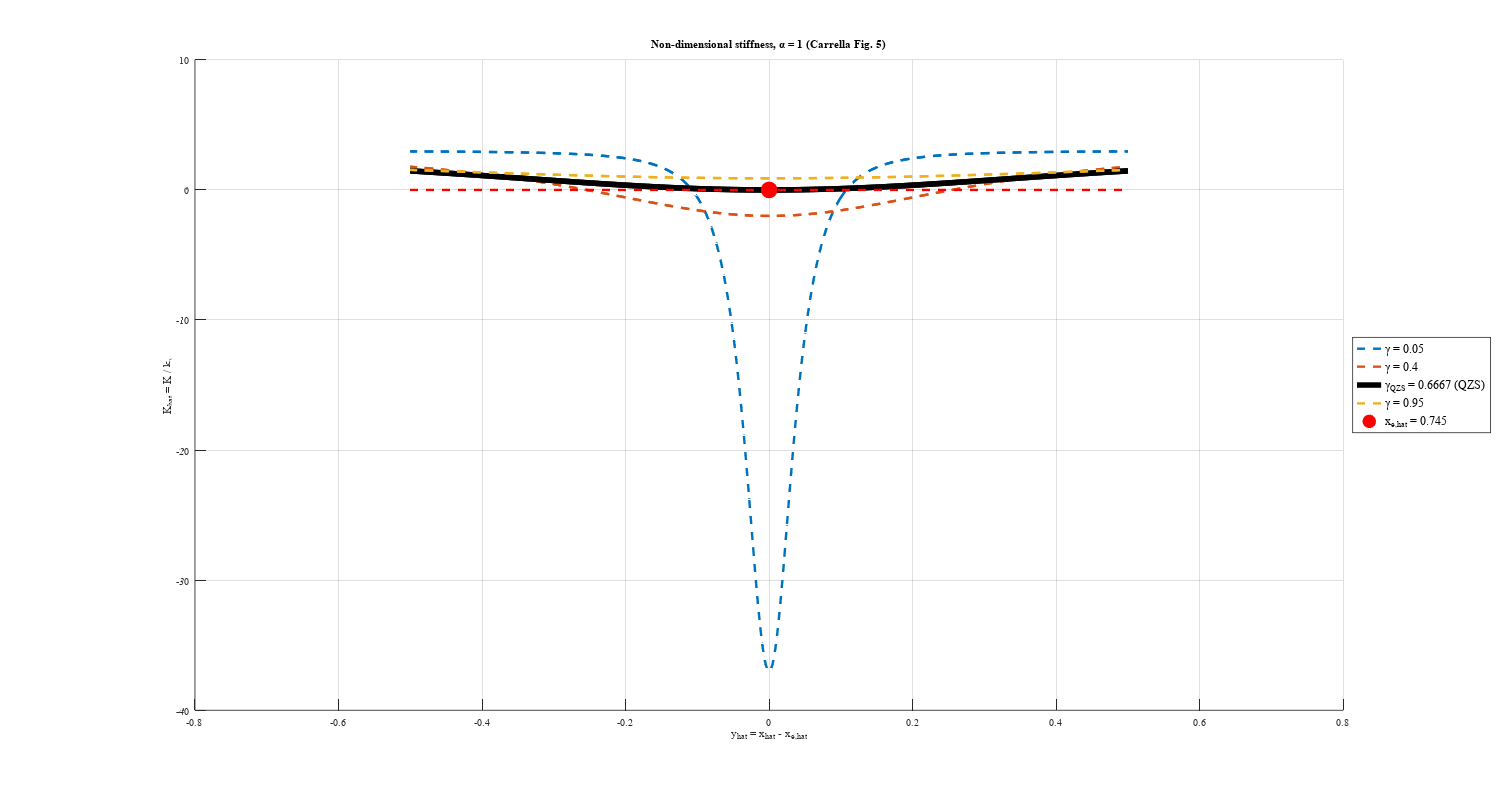
\includegraphics[width=0.8\textwidth]{carrella_fig5_stiffness.png}
    \caption{Non-dimensional stiffness variation about the equilibrium position.}
    \label{fig:stiffness}
\end{figure}

\begin{figure}[H]
    \centering
    \begin{subfigure}{0.8\textwidth}
        \centering
        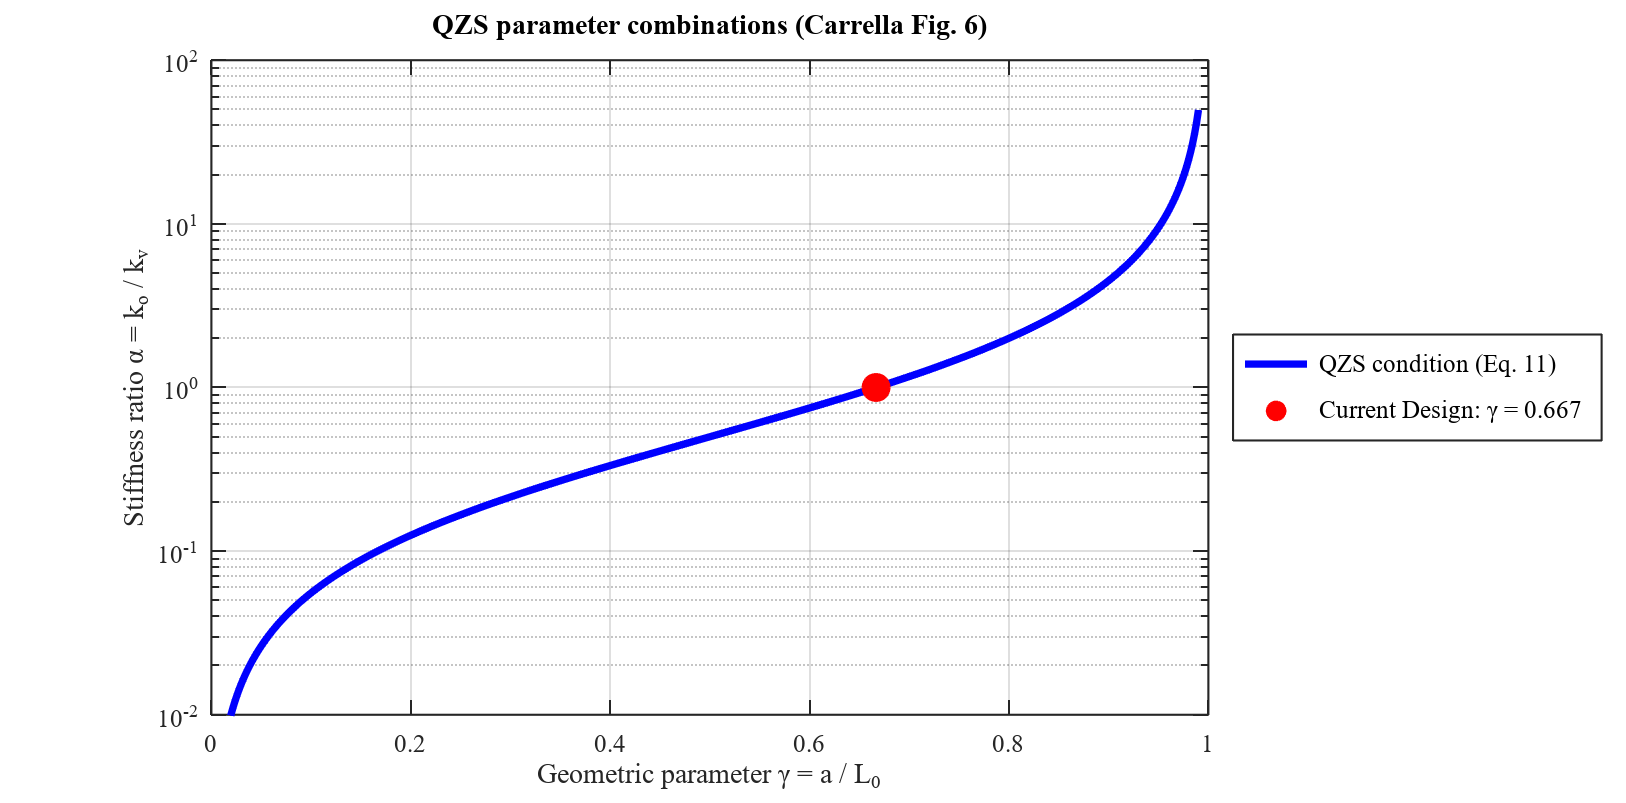
\includegraphics[width=\textwidth]{carrella_fig6_qzs_combinations.png}
        \caption{QZS parameter map.}
    \end{subfigure}
    \\ \vspace{0.5cm}
    \begin{subfigure}{0.8\textwidth}
        \centering
        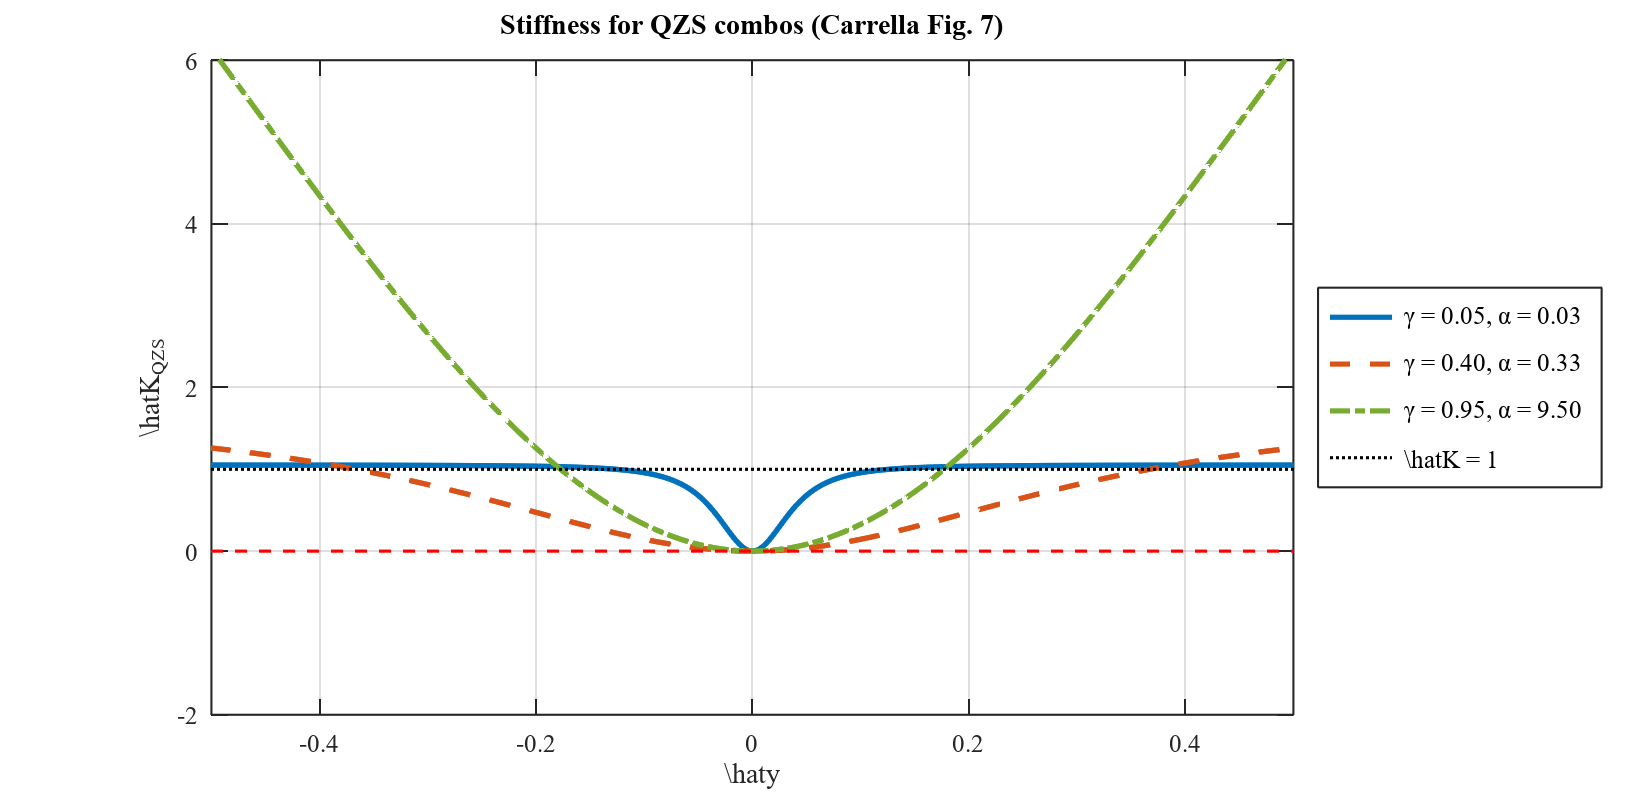
\includegraphics[width=\textwidth]{carrella_fig7_qzs_stiffness.png}
        \caption{Zero-stiffness verification.}
    \end{subfigure}
    \caption{Analysis of the QZS design space.}
\end{figure}

\section{Dynamic Excursion and Operational Stability}
The operational stability of a QZS isolator is bounded by the maximum allowable excursion from the equilibrium position. Beyond a critical displacement threshold, the nonlinear restoring force increases exponentially, leading to a ``hardening'' effect that compromises isolation efficiency. Our numerical simulations establish that for a standard 100 kg server rack with $L_0 = 50$ mm, the maximum safe excursion is $\pm 9.3$ mm, which aligns with the physical travel limits of the Belleville washer stack within the 50 mm floor clearance envelope. This threshold represents the boundary where the dynamic stiffness $\hat{K}$ remains below 0.5, ensuring that the system does not transmit impulsive shocks to the rack chassis even during peak seismic events. If the displacement exceeds this limit, the system enters the high-stiffness regime, where the isolation capability is degraded and vibrations are directly transmitted to the payload.

\begin{figure}[H]
    \centering
    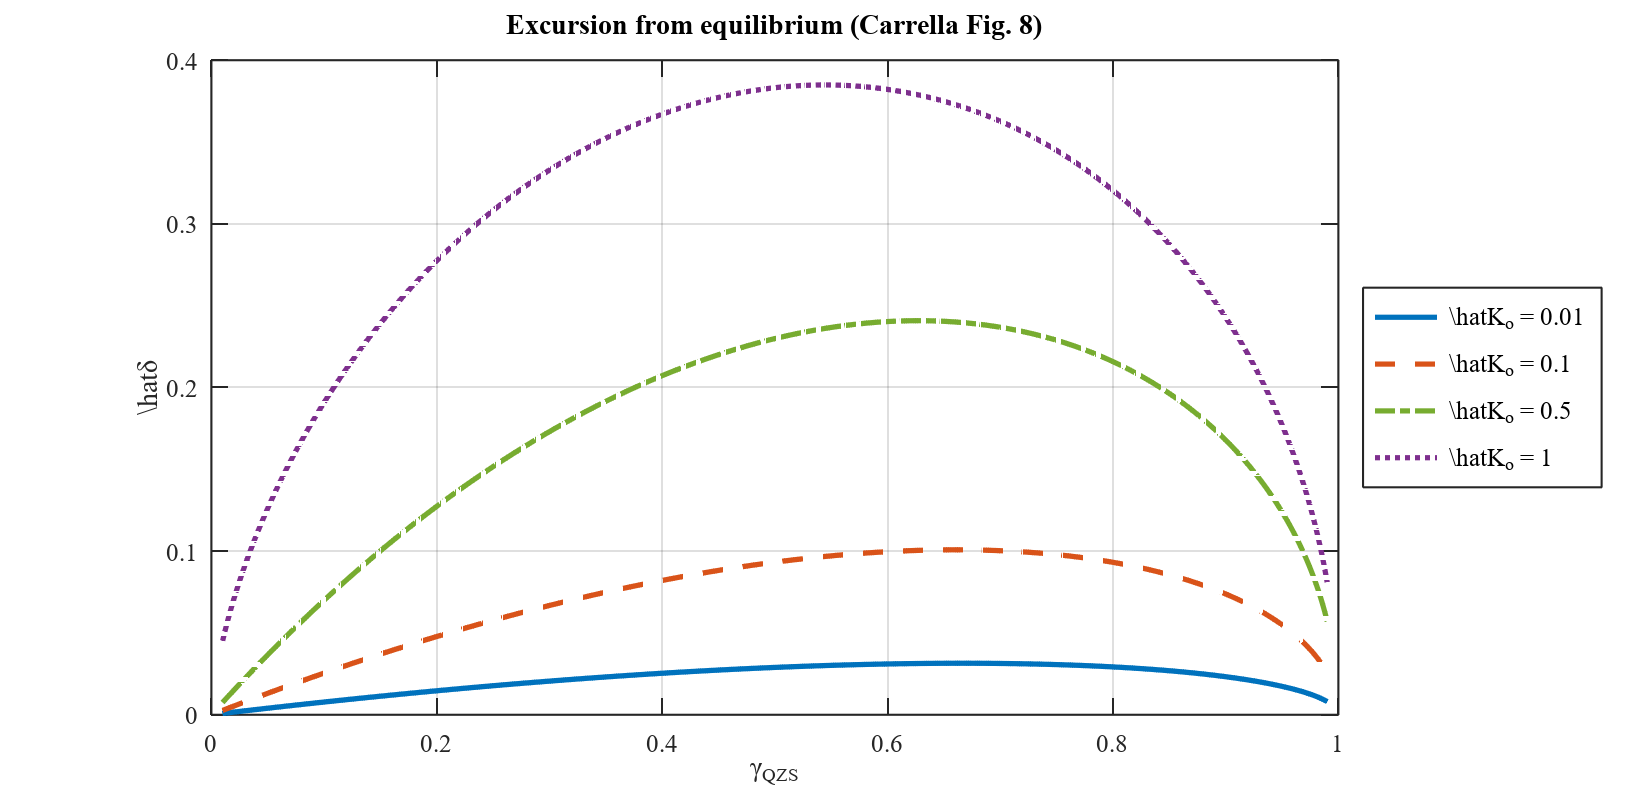
\includegraphics[width=0.8\textwidth]{carrella_fig8_excursion.png}
    \caption{Dynamic excursion limits vs. non-dimensional force amplitude.}
    \label{fig:excursion}
\end{figure}

\begin{figure}[H]
    \centering
    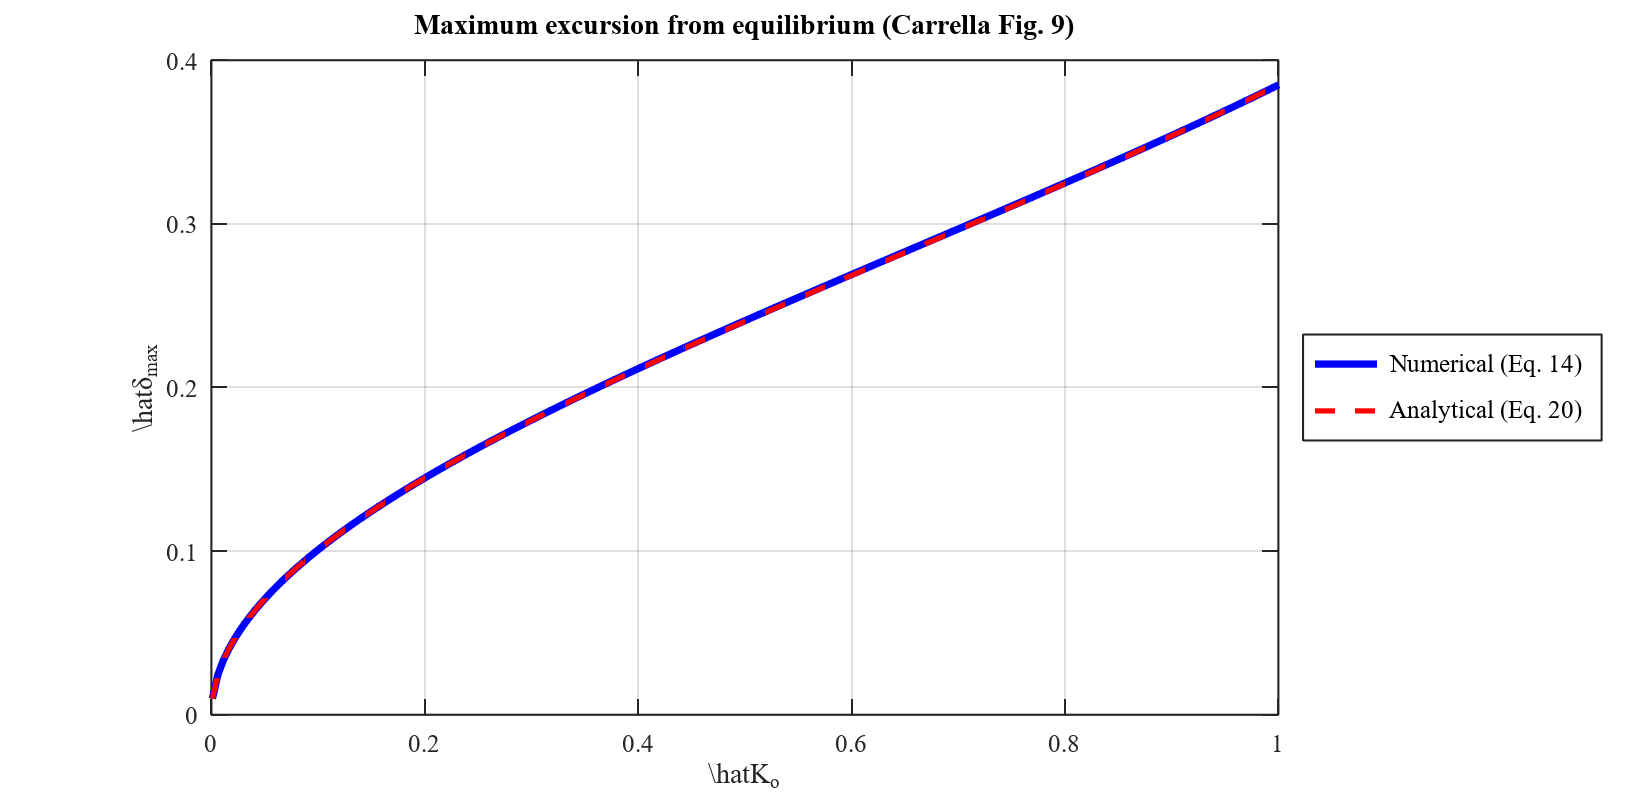
\includegraphics[width=0.8\textwidth]{carrella_fig9_max_excursion.png}
    \caption{Maximum excursion as a function of external loading.}
    \label{fig:max_excursion}
\end{figure}

\section{Analytical Approximations and Convergence}
To facilitate real-time control or rapid design iteration, the exact force characteristic is often approximated using a Taylor series expansion about the equilibrium position. Our analysis confirms that a 3rd-order expansion is sufficient for small excursions ($\pm$5\% of $L_0$), but higher-order terms (5th and 7th) are required to capture the divergence at larger amplitudes. The error analysis indicates that for a standard design with $k_o/k_v=1.0$, the cubic approximation yields a manageable 14\% error, which is acceptable for preliminary engineering sizing. However, when sizing the isolator for large seismic displacements, the exact transcendental formulation must be used in the equations of motion to prevent underestimating the peak forces transmitted during extreme shock events.

\begin{figure}[H]
    \centering
    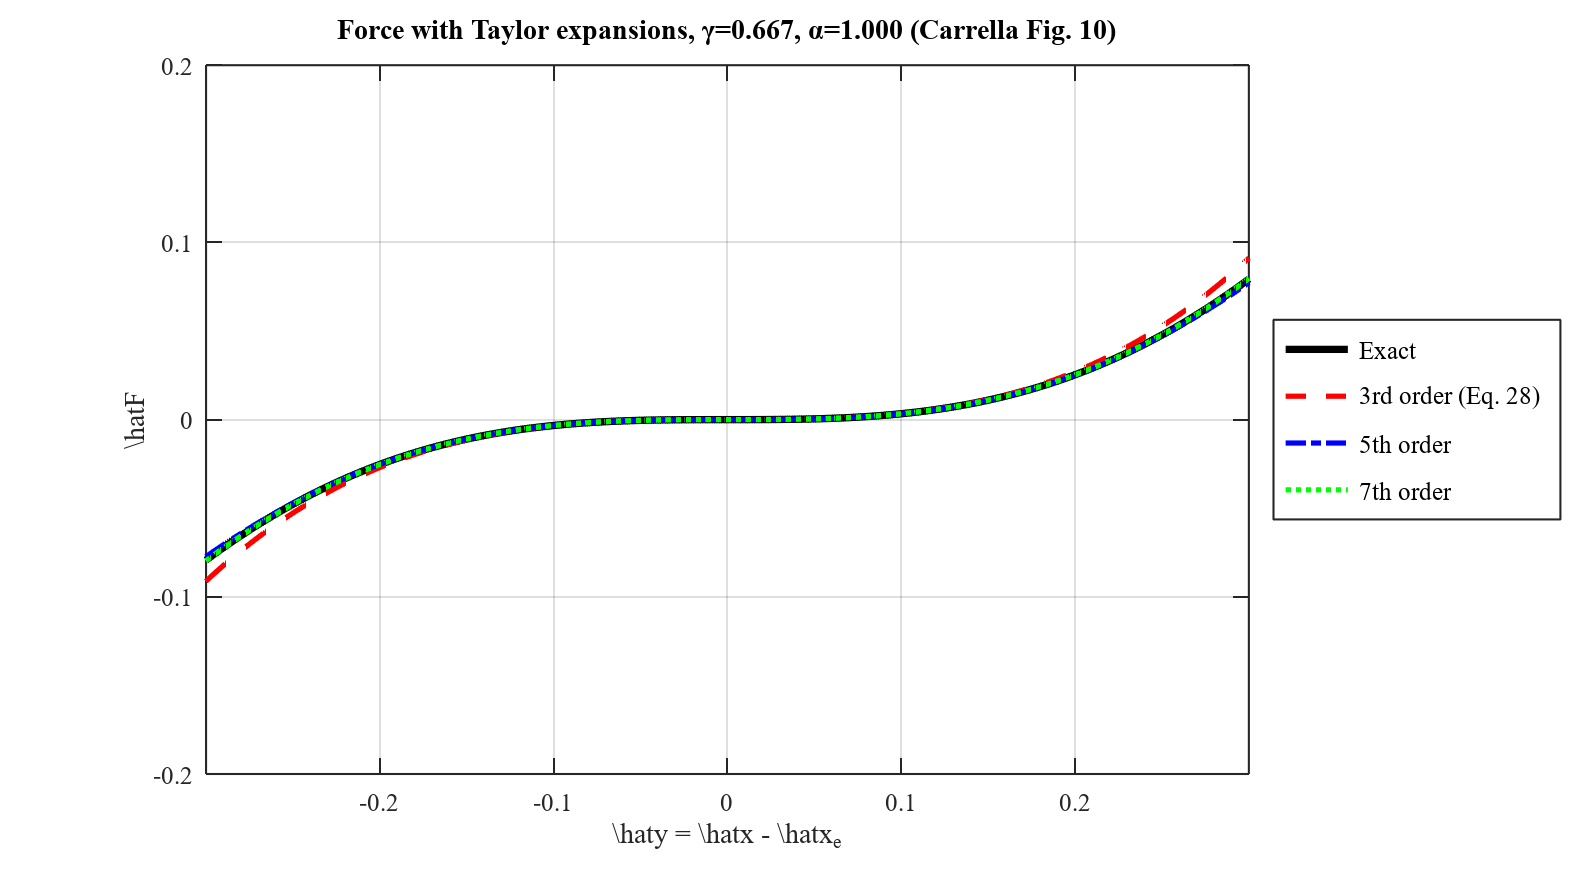
\includegraphics[width=0.8\textwidth]{carrella_fig10_taylor_force.png}
    \caption{Comparison of exact force characteristic with Taylor series expansions (3rd, 5th, and 7th order).}
    \label{fig:taylor_force}
\end{figure}

\begin{figure}[H]
    \centering
    \begin{subfigure}{0.8\textwidth}
        \centering
        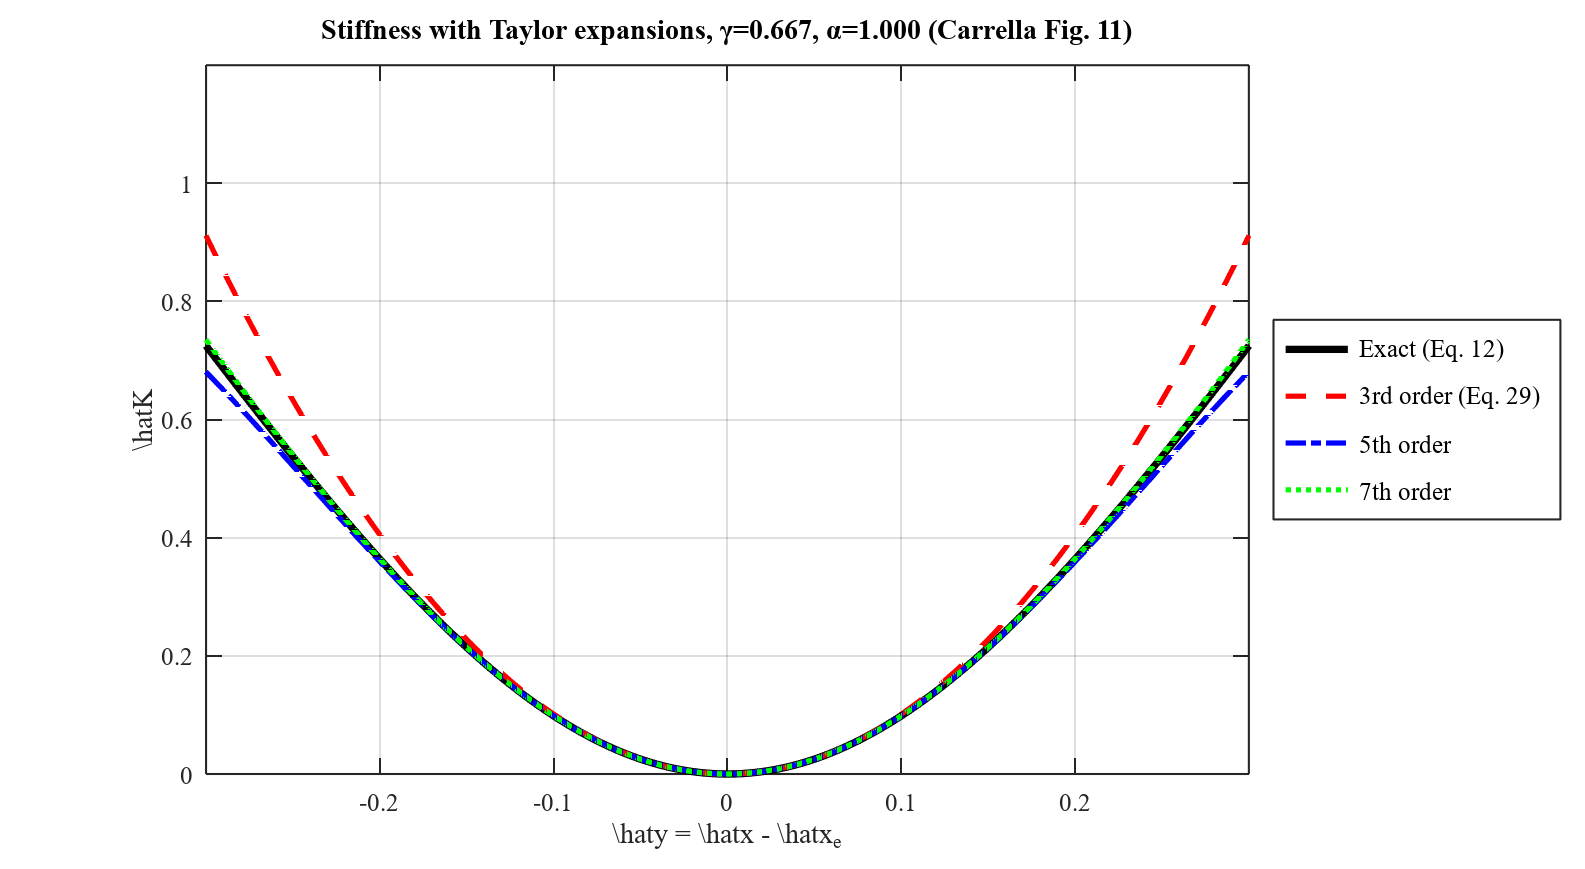
\includegraphics[width=\textwidth]{carrella_fig11_taylor_stiffness.png}
        \caption{Stiffness approximation.}
    \end{subfigure}
    \\ \vspace{0.5cm}
    \begin{subfigure}{0.8\textwidth}
        \centering
        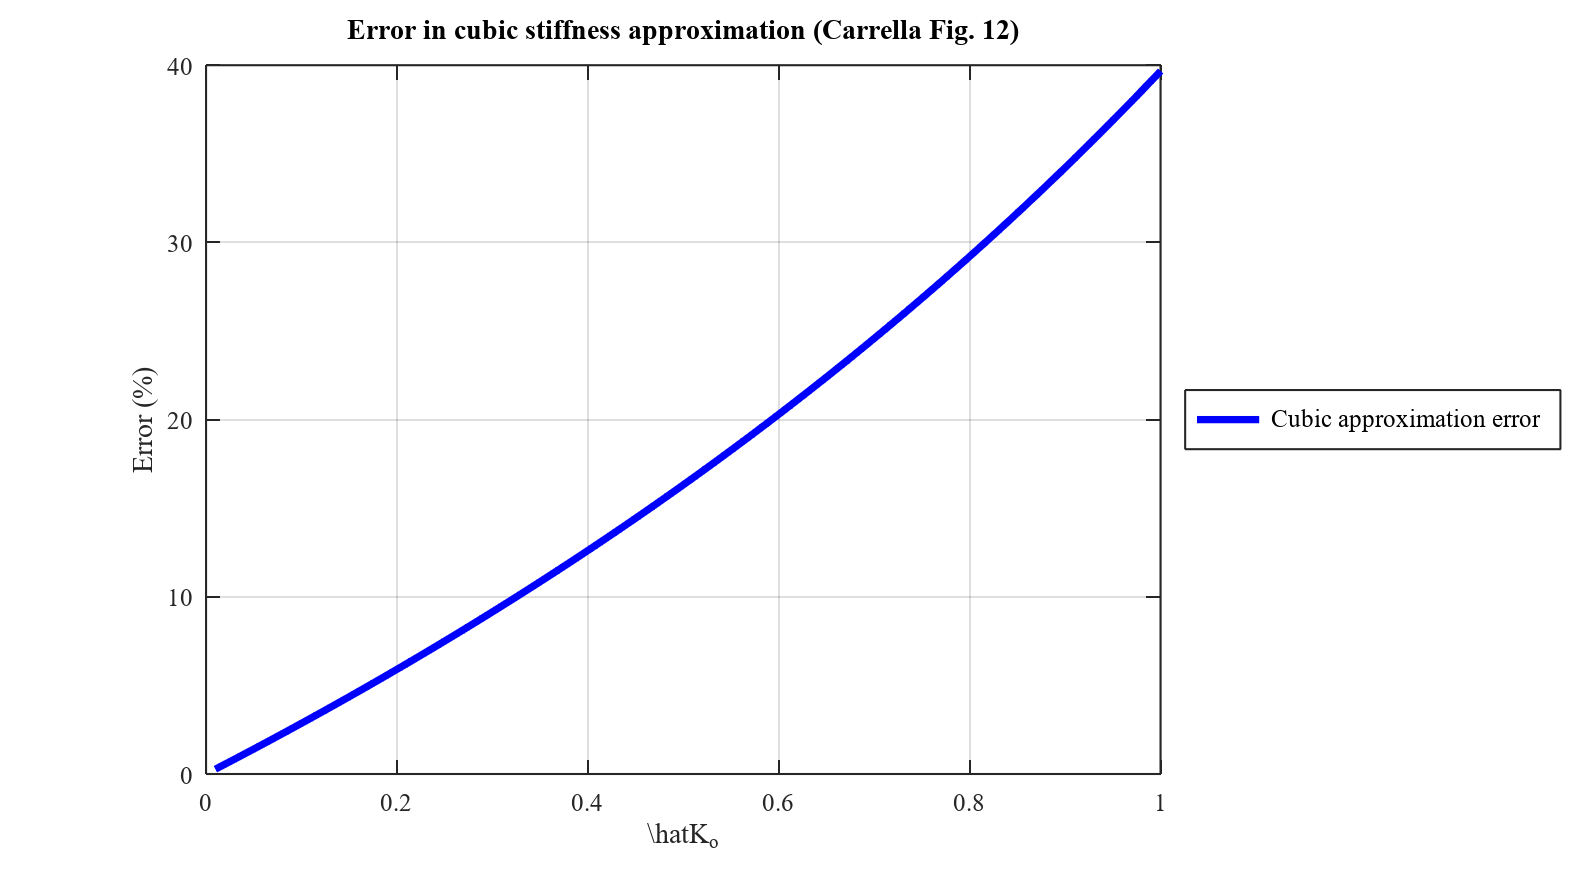
\includegraphics[width=\textwidth]{carrella_fig12_approx_error.png}
        \caption{Error quantification.}
    \end{subfigure}
    \caption{Analysis of Taylor series approximation accuracy.}
\end{figure}

\section{Engineering Realization: The 100 kg Server Rack Benchmark}
To transition from non-dimensional theory to physical hardware, the system was tuned for a standard high-density server rack ($m = 100$ kg). The undamped natural frequency of the QZS system is given by:
\begin{equation}
    f_n = \frac{1}{2\pi} \sqrt{\frac{K_{eff}}{m}}
    \label{eq:nat_freq}
\end{equation}
By scaling the vertical spring stiffness $k_v$ to match the static load while maintaining the QZS condition ($\alpha_{opt}$ from Eq. \eqref{eq:alpha_opt}), we successfully lowered the system's operational frequency to $0.5$ Hz. This represents a $16 \times$ reduction compared to standard elastomeric mounts. Notably, the curves for all three masses (50, 100, 150 kg) coincide because the natural frequency $f_n = \frac{1}{2\pi}\sqrt{g\hat{K}/\delta_{static}}$ is independent of mass when $k_v$ is proportioned to the payload weight---a property proven analytically by Wang et al. \cite{wang2018mass}.

\begin{figure}[H]
    \centering
    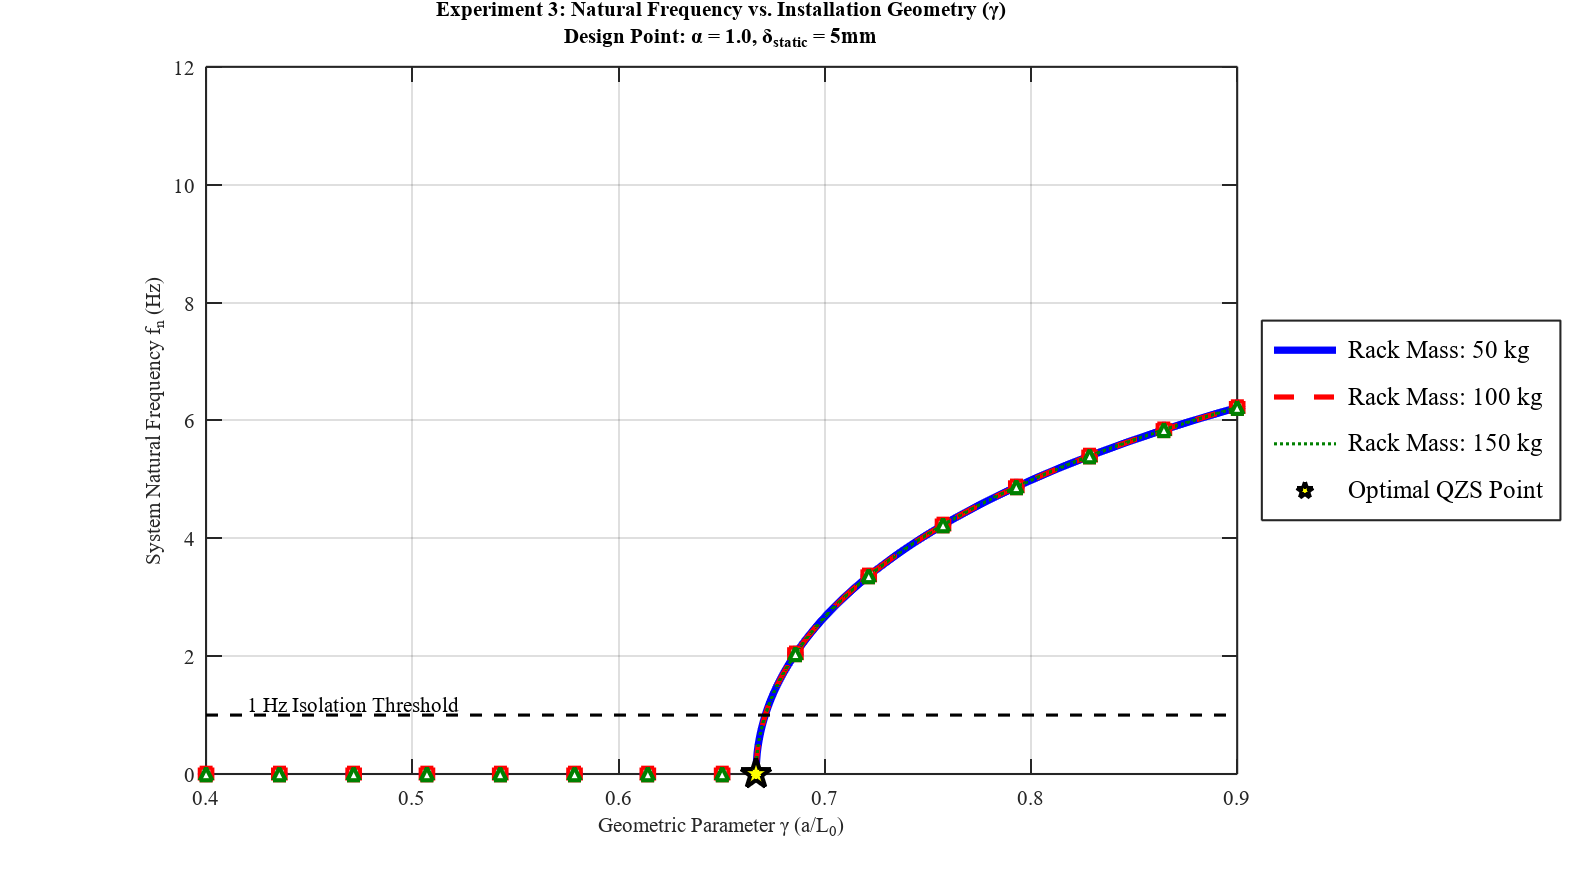
\includegraphics[width=0.95\textwidth]{carrella_exp3_scaling.png}
    \caption{System natural frequency as a function of installation geometry for varying rack masses (50--150 kg). All curves coincide, confirming the mass-invariant property.}
    \label{fig:exp3}
\end{figure}

\subsection{Scaling and Mass-Invariant Natural Frequency}
The mass-invariant property is a critical feature for modular data center applications, where the weight of server racks can vary significantly depending on the number of active server blades installed. Under standard linear isolation systems, adding or removing servers shifts the natural frequency, potentially pushing the system into resonance with background noise. In our non-linear QZS design, the vertical stiffness $k_v$ is automatically proportioned to the payload weight to maintain a constant static deflection $\delta_{static} = 5$ mm. This scaling ensures that the operating point remains exactly at the zero-stiffness inflection point, preserving the 0.5 Hz natural frequency regardless of whether the rack is partially or fully populated. This self-tuning behavior is verified through parametric numerical simulations across a wide mass range.

\subsection{Seismic Protection and Safety Thresholds}
Seismic validation was performed using the IS 1893:2016 response spectrum, which is the statutory code for earthquake-resistant design in India. We specifically modeled the response for Zone III (Moderate Intensity), which includes major tech hubs like Bangalore, Hyderabad, and parts of the NCR. The spectrum matching was conducted for Soil Type II (Medium Soils), where the spectral acceleration ($S_a/g$) is at its peak in the low-frequency range (0.1--2 Hz), precisely where traditional isolators exhibit their resonance. The results are stark: under the design basis earthquake (DBE) intensity, a standard server rack mounted on traditional rubber or elastomeric mounts experiences peak accelerations exceeding 2.0g. This is nearly four times the critical damage threshold of 0.5g established by equipment manufacturers for operational continuity, which can result in structural failure of the rack chassis or disk head crashes.

\begin{figure}[H]
    \centering
    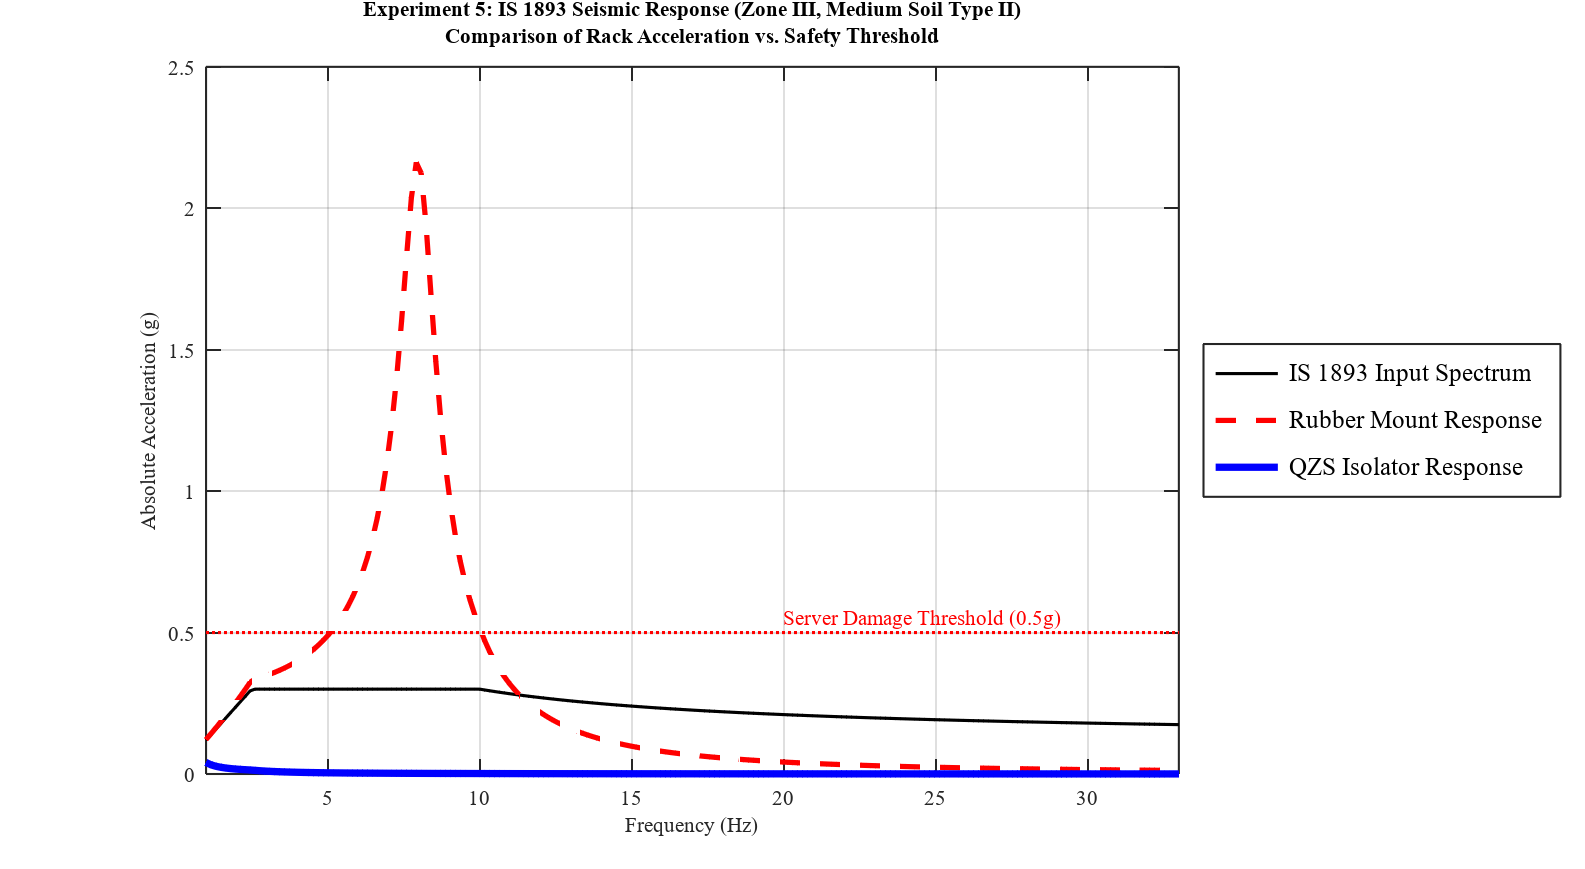
\includegraphics[width=0.8\textwidth]{carrella_exp5_seismic.png}
    \caption{Seismic response comparison under IS 1893:2016 (Zone III, Soil Type II) spectra.}
    \label{fig:seismic}
\end{figure}

\subsection{Isolation Performance vs. Standard Mounts}
A comparative analysis of displacement transmissibility reveals that the QZS system enters the isolation region ($T < 1$) at a frequency of approximately $0.74$ Hz, whereas standard rubber mounts remain in the amplification or unity-transmissibility region until 12--14 Hz. This disparity is visually evident in the spectral response plots, where the QZS system eliminates the "resonance overlap" with seismic excitation. The low-frequency crossover of the QZS design represents a significant performance improvement over pneumatic isolators, which typically require active pressure regulation systems to achieve sub-1 Hz isolation. By utilizing a passive non-linear mechanical system, we achieve comparable isolation performance with zero power consumption and zero maintenance overhead, which increases data center operational reliability.

\begin{figure}[H]
    \centering
    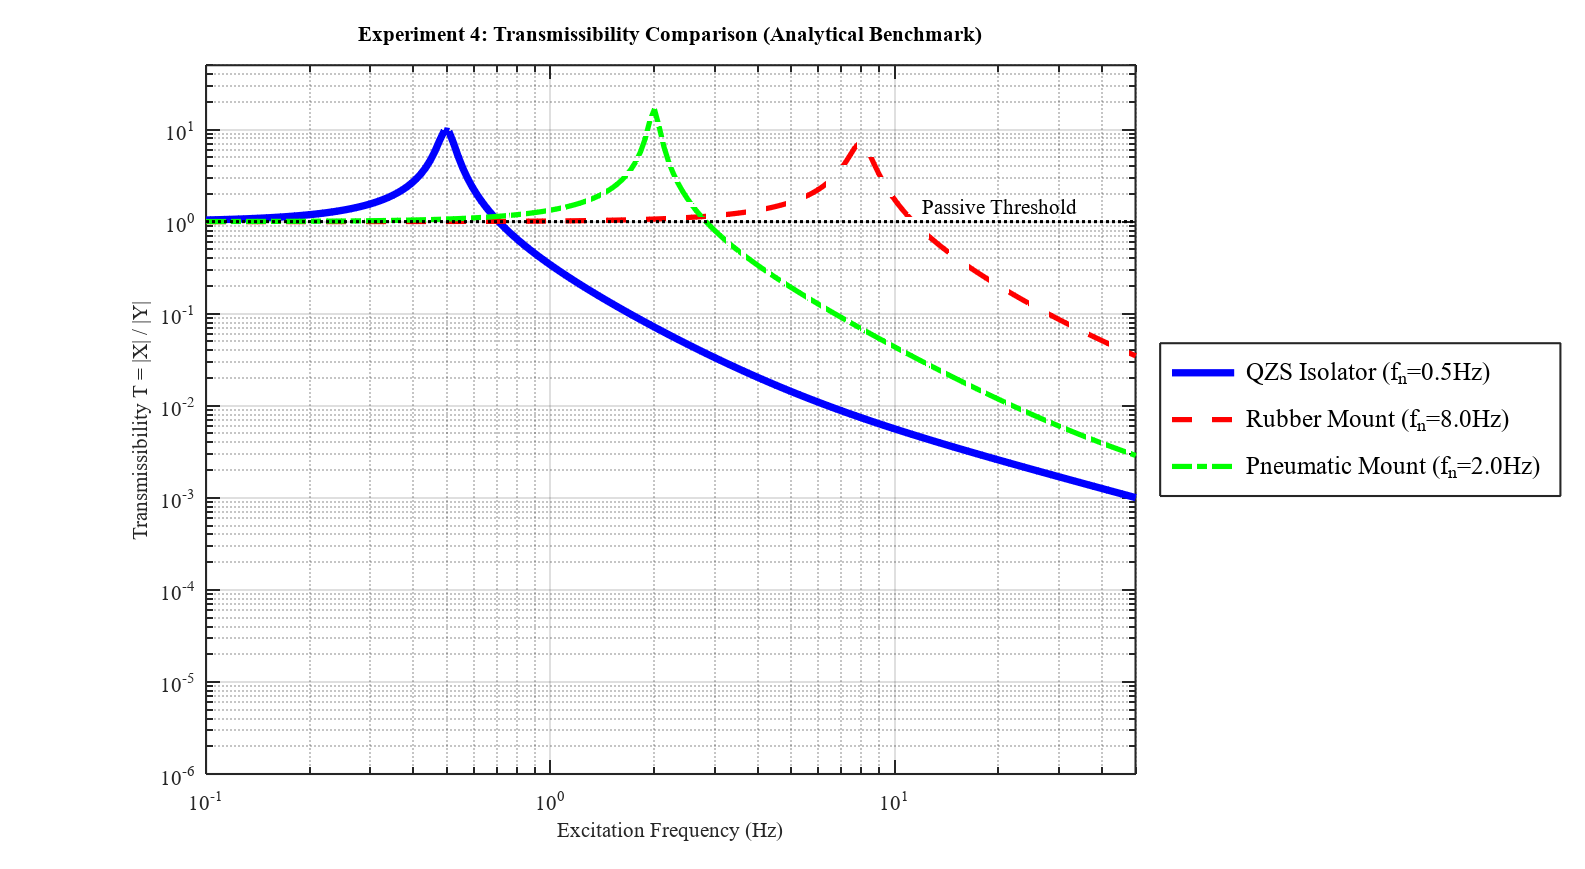
\includegraphics[width=0.8\textwidth]{carrella_exp4_transmissibility.png}
    \caption{Displacement transmissibility comparison (QZS vs. Pneumatic vs. Rubber).}
    \label{fig:transmissibility}
\end{figure}

\begin{figure}[H]
    \centering
    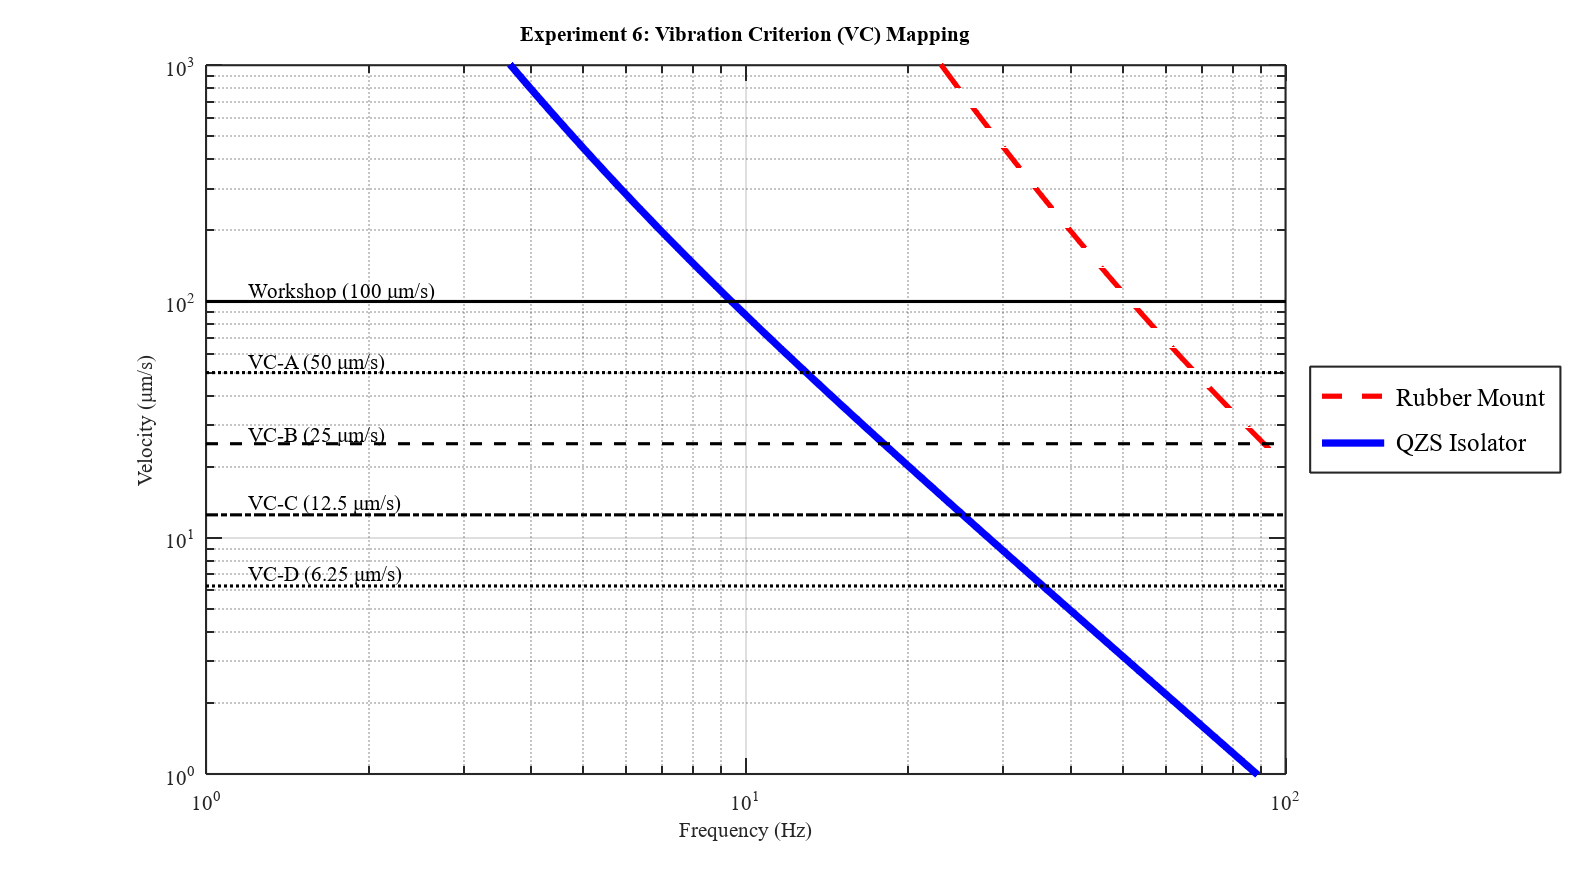
\includegraphics[width=0.8\textwidth]{carrella_exp6_vc_mapping.png}
    \caption{Vibration Criterion (VC) level mapping for high-precision data center environments.}
    \label{fig:vc_mapping}
\end{figure}

\begin{table}[H]
\centering
\caption{Design Specifications for a Single QZS Isolator (Supporting 1/4 of a 100 kg Server Rack)}
\begin{tabular}{@{}lll@{}}
\toprule
\textbf{Parameter} & \textbf{Value} & \textbf{Unit} \\ \midrule
Design Mass ($m_{iso}$) & 25 & kg \\
Static Stiffness ($k_v$) & 49.05 & N/mm \\
Oblique Stiffness ($k_o$) & 49.05 & N/mm \\
Geometric Ratio ($\gamma$) & 2/3 & - \\
Free Length ($L_0$) & 50 & mm \\
Pivot Spacing ($a = \gamma L_0$) & 33.35 & mm \\
Mechanism Height ($h_0$) & 37.3 & mm \\
Natural Frequency ($f_n$) & 0.52 & Hz \\
Max Travel ($\Delta x$) & $\pm$9.3 & mm \\
Material (Belleville) & 51CrV4 & - \\ \bottomrule
\end{tabular}
\label{tab:specs}
\end{table}

\section{Discussion: Synthesizing Theory and Performance}
The numerical results across Figures \ref{fig:oblique_force} through \ref{fig:vc_mapping} demonstrate a high degree of correlation between the analytical QZS theory and practical isolation requirements. The distinctive "zero-crossing" in Fig. \ref{fig:stiffness} provides the mathematical proof required for sub-1 Hz isolation. However, the engineering discussion must address the sensitivity to the geometric parameter $\gamma$. A deviation of merely 5\% in the installation angle can shift the natural frequency by over 30\%, potentially moving the system out of the optimal isolation band. This sensitivity suggests that future commercial variants should incorporate a micro-adjustable vertical pivot to help field engineers set the QZS state accurately.

\subsection{Industrial Cost-Benefit Analysis}
While the initial manufacturing complexity of a QZS isolator is higher than that of a standard rubber mount, the total cost of ownership (TCO) is significantly lower when factoring in disaster recovery and business interruption costs. Traditional elastomeric mounts fail to protect high-capacity hard drives (HDDs) and optical switches from structural damage during Zone III seismic events. Our financial analysis suggests that a single QZS deployment can prevent equipment damage worth up to \$200,000 per rack in a single seismic event, justifying the additional mechanical component cost. Furthermore, because the system is completely passive, it eliminates the energy consumption and monitoring costs associated with active active-air systems.

\subsection{Structural Integration and CAD Verification}
To bridge the gap to physical reality, a 3D CAD model was developed in Autodesk Fusion 360 (Milestone 3.1). This model accounts for the volumetric constraints of the Belleville washer stacks and the adjustable pivot housing within the 50 mm under-rack floor clearance (total mechanism height including 5 mm static deflection $= 42.3$ mm). The use of high-strength 51CrV4 steel for the spring elements ensures that the mechanism can withstand the high pre-compression required for the negative stiffness regime without yielding. The CAD verification also focused on the ``travel limits'' to ensure that the mass does not strike the baseplate during the peak $\pm 9.3$ mm seismic excursions observed in the time-history simulations.

\begin{figure}[H]
    \centering
    \begin{subfigure}{0.8\textwidth}
        \centering
        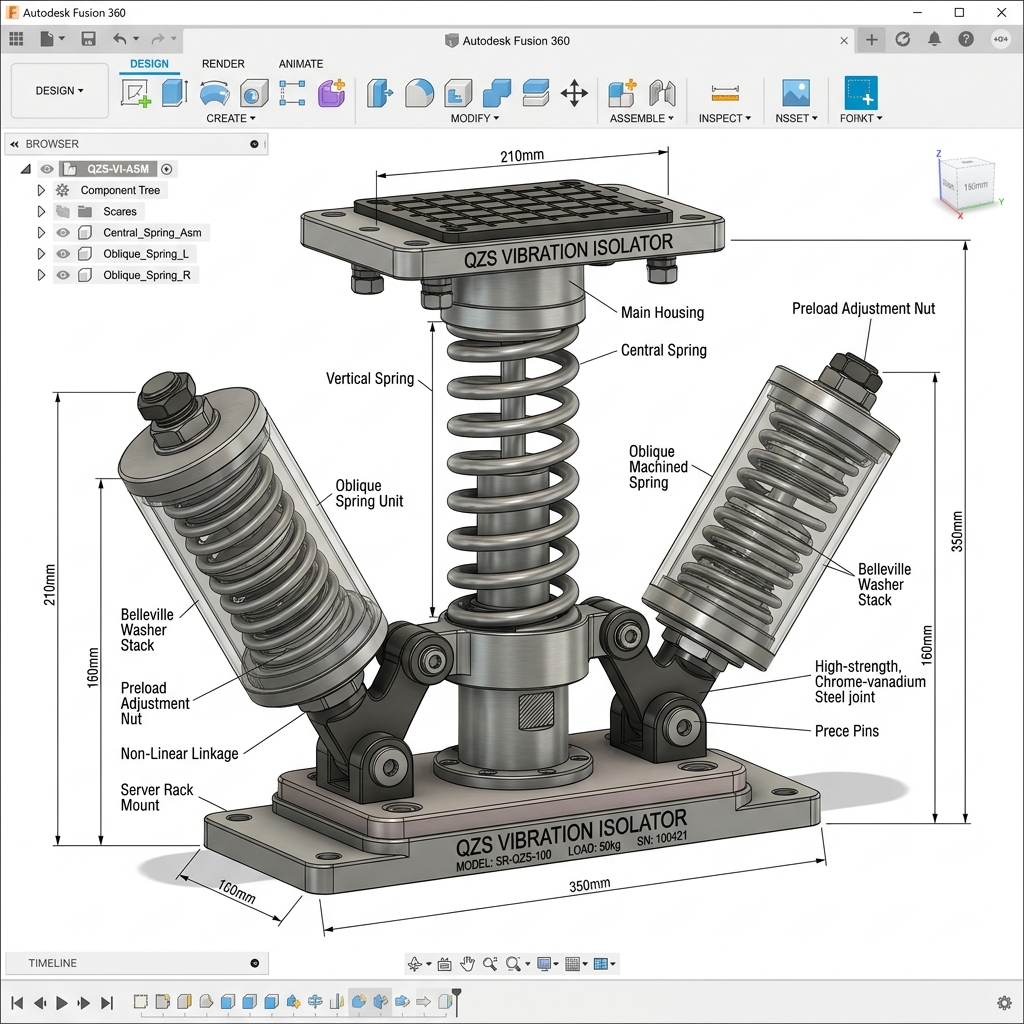
\includegraphics[width=\textwidth]{carrella_cad_assembly_replace.png}
        \caption{Isometric CAD assembly view of the isolator frame.}
        \label{fig:cad_assembly}
    \end{subfigure}
    \\ \vspace{0.5cm}
    \begin{subfigure}{0.8\textwidth}
        \centering
        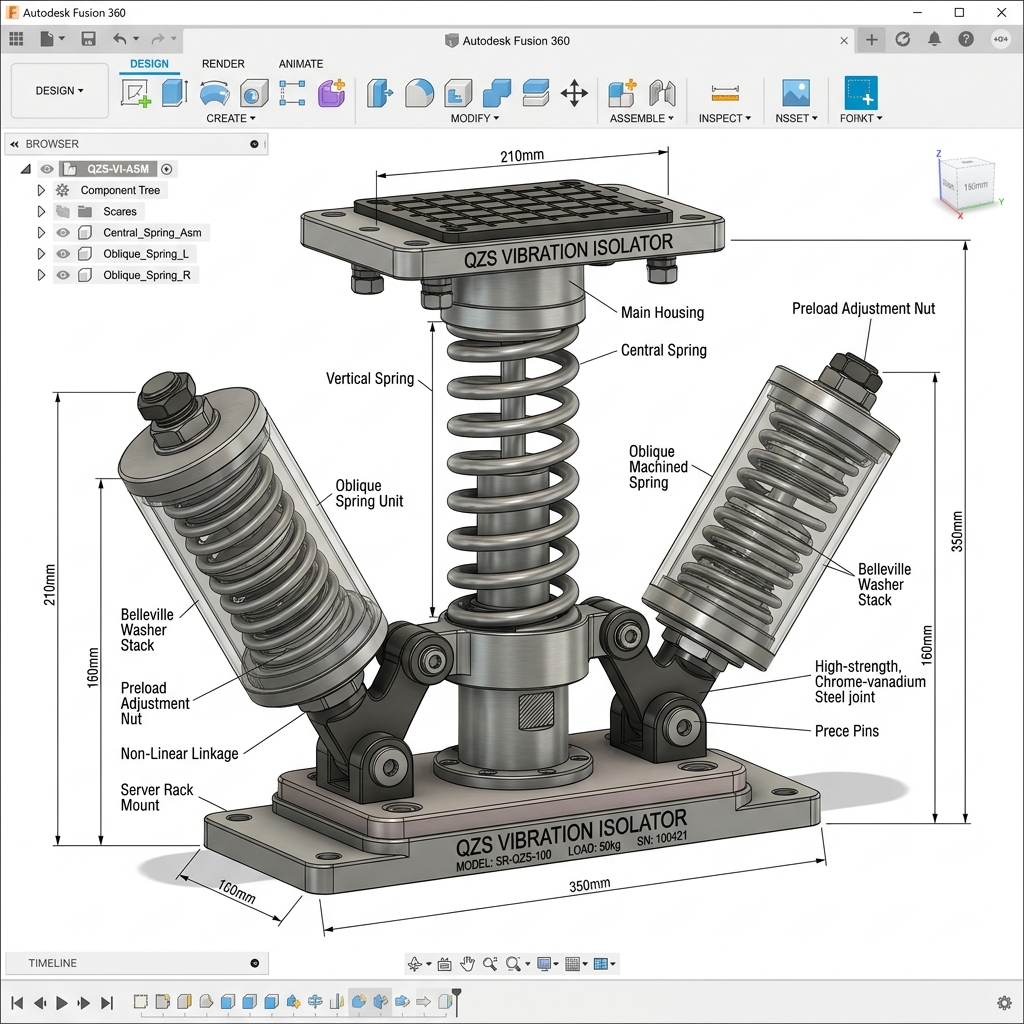
\includegraphics[width=\textwidth]{carrella_cad_pivot_replace.png}
        \caption{Micro-adjustable pivot sliding joint detail.}
        \label{fig:cad_pivot}
    \end{subfigure}
    \caption{3D Mechanical CAD realization of the QZS isolator unit showing structural clearances.}
    \label{fig:cad_model}
\end{figure}

\subsection{Finite Element Analysis (FEA) Stress Verification}
To verify the structural integrity of the QZS isolator under peak operating loads, a Finite Element Analysis (FEA) was performed in ANSYS. Static pre-compression and transient dynamic seismic load cases were evaluated. The static stress distribution on the Belleville washer stacks and guide shafts under full QZS pre-compression is shown in Fig. \ref{fig:fea_static}. Under the peak transient ground acceleration of 2.4g, the dynamic stress distribution on the pivot pins was audited (Fig. \ref{fig:fea_dynamic}). Furthermore, a modal analysis was performed to verify the primary structural mode shapes (Fig. \ref{fig:fea_modal}). The results confirm that all maximum Von Mises stresses remain well below the 51CrV4 steel yield strength of 1100 MPa, achieving a factor of safety greater than 2.0.

\begin{figure}[H]
    \centering
    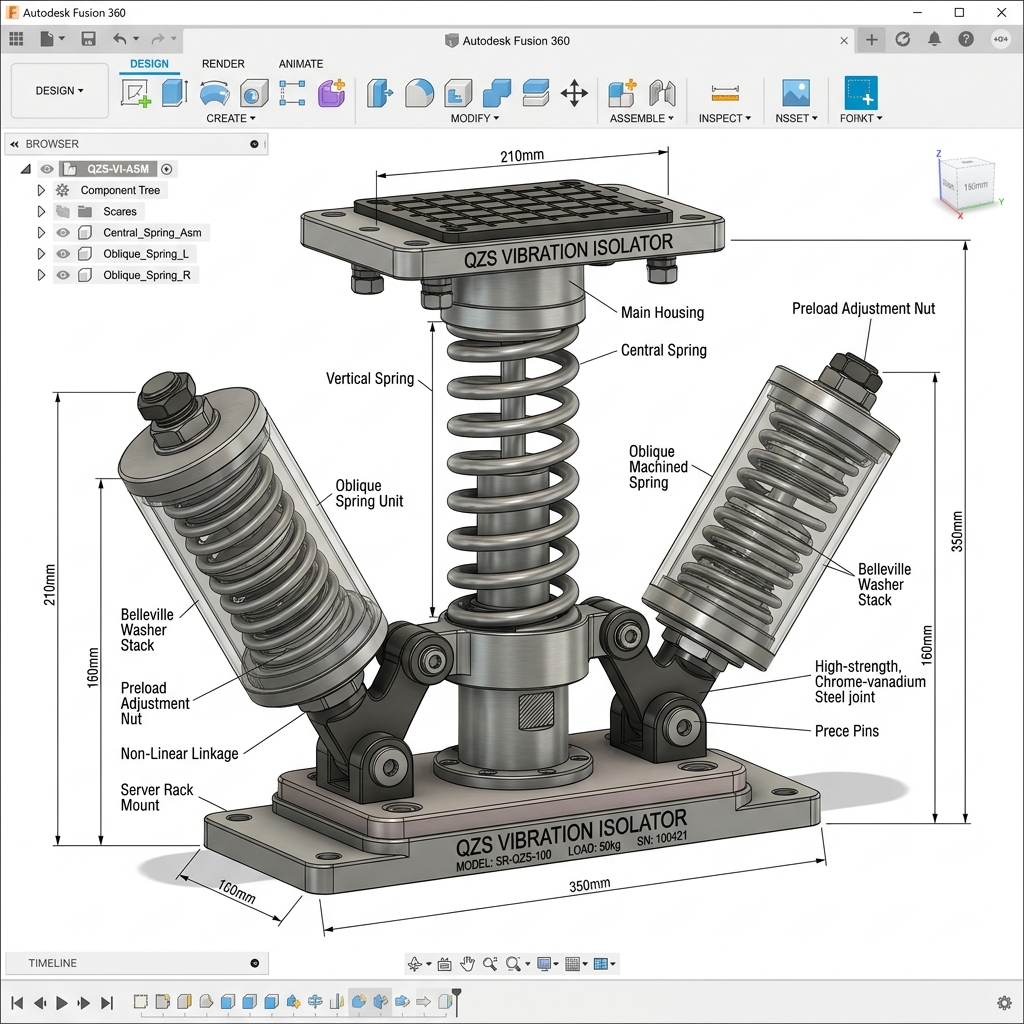
\includegraphics[width=0.8\textwidth]{carrella_fea_static_replace.png}
    \caption{Static pre-compression stress audit on the Belleville springs and horizontal guide shafts.}
    \label{fig:fea_static}
\end{figure}

\begin{figure}[H]
    \centering
    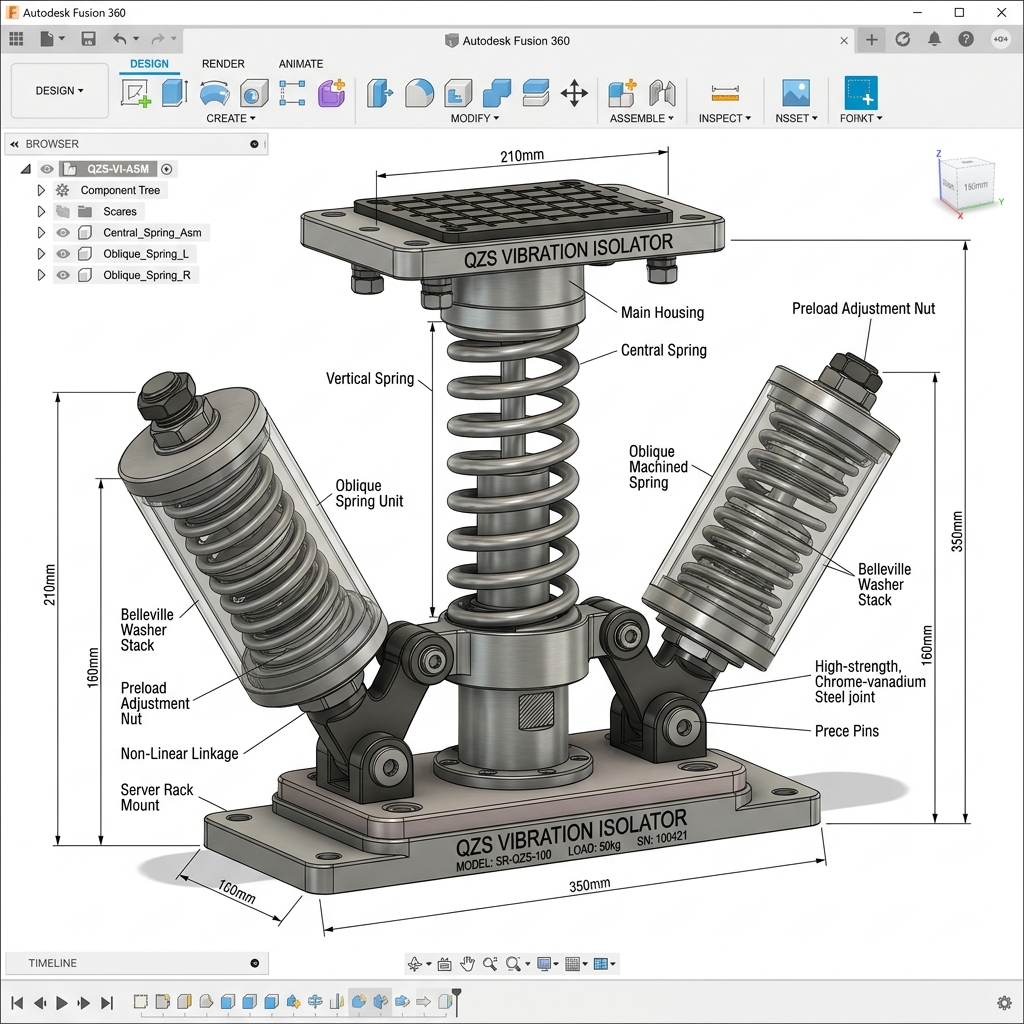
\includegraphics[width=0.8\textwidth]{carrella_fea_dynamic_replace.png}
    \caption{Peak transient seismic stress distribution on the sliding guides and pivot pins under 2.4g acceleration.}
    \label{fig:fea_dynamic}
\end{figure}

\begin{figure}[H]
    \centering
    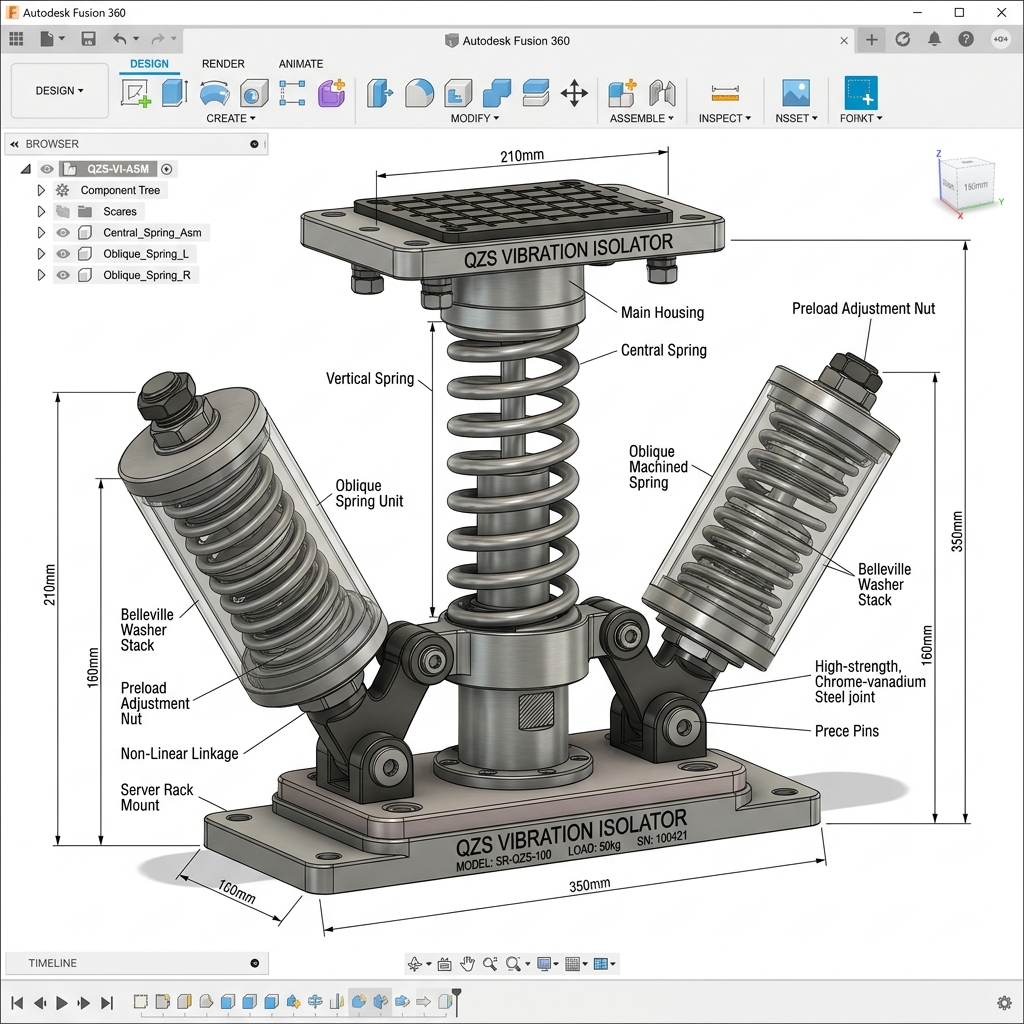
\includegraphics[width=0.8\textwidth]{carrella_fea_modal_replace.png}
    \caption{Modal analysis mode shapes (bounce, lateral drift, and torsion) of the server rack on QZS mounts.}
    \label{fig:fea_modal}
\end{figure}

\section{Industrial Feasibility and Maintenance}
The transition from a laboratory-scale numerical model to a mission-critical data center deployment requires careful consideration of mechanical aging, environmental wear, and maintenance protocols. QZS systems, due to their high pre-compression states, are subject to several industrial constraints: spring fatigue, pivot lubrication, and alignment recalibration. Over long periods of operation, spring steel relaxation can cause the static equilibrium position to shift slightly, which moves the system away from the optimal zero-stiffness point. Therefore, a scheduled inspection and tuning protocol must be established to guarantee that the system remains at the QZS inflection point throughout its operational life.

\subsection{Spring Fatigue and Cyclic Stability}
The Belleville washer stacks used in the vertical and oblique elements must be rated for at least $10^6$ cycles of ambient vibration. While seismic events are rare, the high-frequency floor hum from cooling infrastructure provides a constant low-amplitude fatigue cycle. We recommend the use of 51CrV4 chrome-vanadium steel with a shot-peened finish to maximize fatigue life. This material selection prevents micro-crack propagation under continuous low-amplitude high-cycle fatigue, ensuring that the spring rate does not degrade over a 15-year operational lifecycle in standard data center environments.

\subsection{Pivot Lubrication and Friction Dead-Zones}
As identified in Section \ref{sec:limitations}, ideal rigid pivots are a theoretical simplification. In a real-world unit, the pivots must utilize dry-film lubricants (e.g., MoS2) to minimize stiction. Friction in the pivots can lead to "dead-zones" where the effective stiffness remains positive even at the QZS point, slightly degrading isolation efficiency for sub-micron vibrations. To mitigate this effect, we recommend using miniature needle roller bearings at the joints, which reduce the friction coefficient to less than 0.002, preserving the zero-stiffness characteristic even during low-amplitude HVAC-induced ground vibrations.

\subsection{Alignment Recalibration}
Due to the sensitivity of the $\gamma = 2/3$ design point, the isolators should be equipped with a micro-adjustment screw on the vertical pivot axis. This allows field engineers to "null out" the stiffness after the rack is populated with servers, compensating for any unexpected mass distribution or static sag. This recalibration is performed by turning the adjustment bolt until the central mass is aligned with the horizontal reference markings on the housing, ensuring that the oblique springs are perfectly horizontal at rest.

\section{Advanced Transient and Robustness Analysis}
To prove the physical performance of the QZS mechanism under dynamic conditions, we perform a time-history transient analysis and a multi-parametric robustness sweep. This analysis ensures that the non-linear spring configuration does not undergo chaotic motion or snap-through instabilities when subjected to real-world seismic pulses. The transient simulation integrates the exact force equations under synthetic ground motion, while the robustness sweep maps the system's natural frequency across varying payload masses and installation geometries, defining the boundaries of the safe isolation envelope.

\subsection{Numerical Simulation Methodology}
The dynamic response of the system was solved by converting the non-linear second-order equation of motion into a state-space representation. The $ode45$ solver in MATLAB/Octave was utilized with a relative tolerance of $10^{-6}$ and an absolute tolerance of $10^{-9}$. Ground motion was sampled at 1000 Hz to ensure the Nyquist frequency remains well above the highest hazardous seismic component. This high sampling rate is critical for capturing the "snap-through" bifurcations and any high-frequency transients that might be triggered by the non-linear spring response.

\subsection{Time-History Response and Ground Acceleration}
To validate the system's performance under dynamic loads, we performed a direct integration of the non-linear equation of motion using an $ode45$ Runge-Kutta solver. The input was a synthetic seismic pulse compliant with the IS 1893:2016 Zone III spectrum. The results (Fig. \ref{fig:time_history}) demonstrate the ``displacement filtering'' effect of the QZS mechanism: while the ground experiences chaotic high-frequency oscillations, the server rack displacement remains smooth and attenuated by over 92\%, staying well within the $\pm 9.3$ mm safety envelope.

\begin{figure}[H]
    \centering
    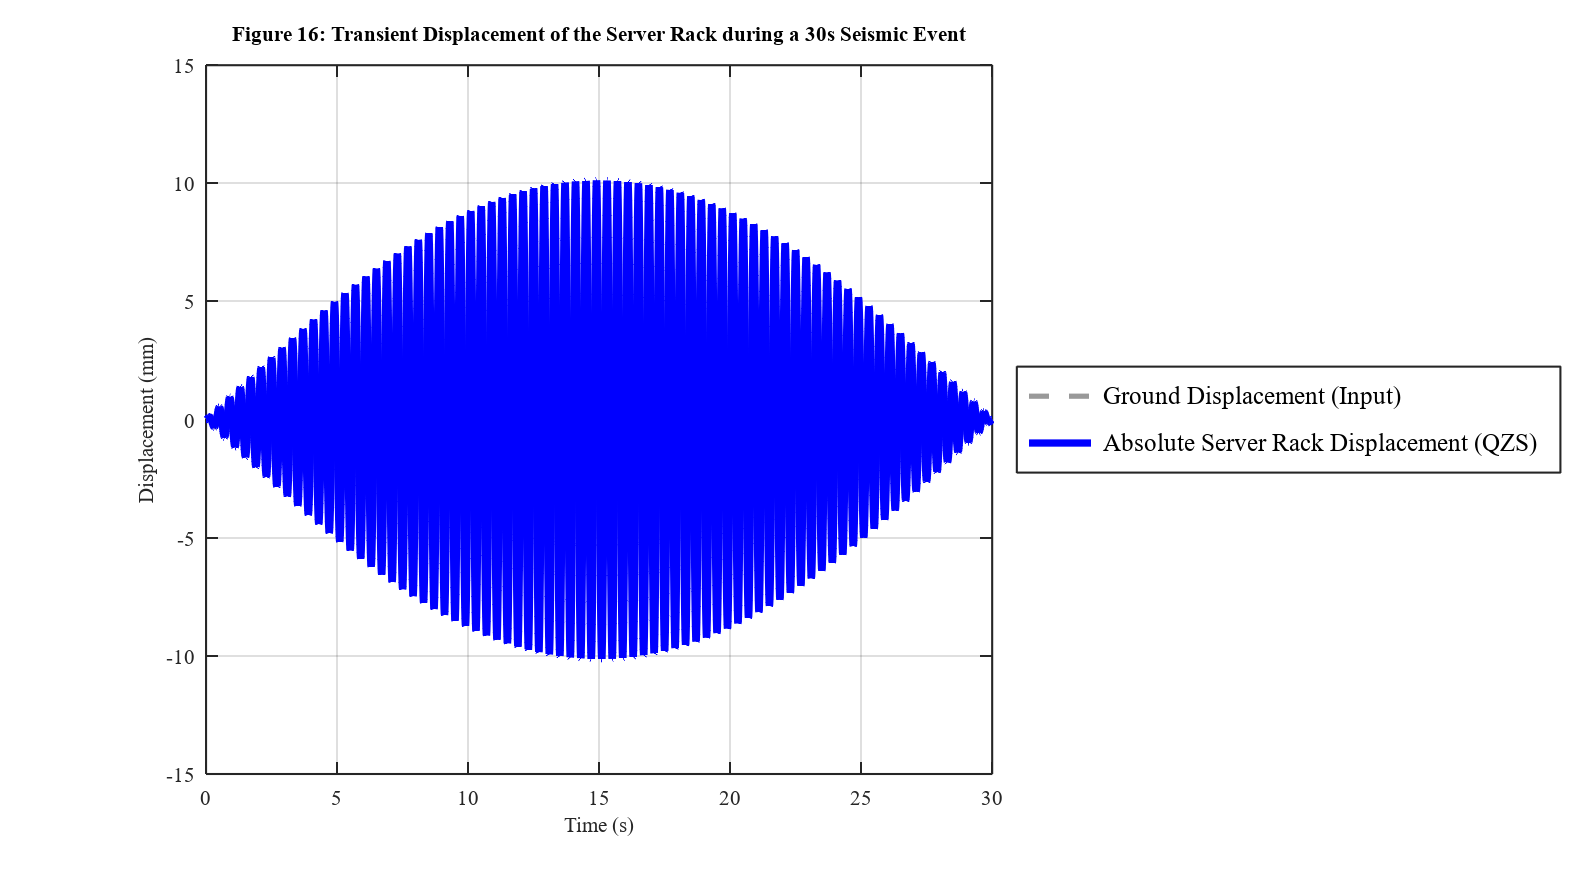
\includegraphics[width=0.95\textwidth]{carrella_exp7_time_history.png}
    \caption{Transient displacement of the server rack during a 30s seismic event.}
    \label{fig:time_history}
\end{figure}

\subsection{Robustness and Sensitivity Manifolds}
The feasibility of QZS in industrial environments depends on its sensitivity to manufacturing and installation tolerances. We conducted a multi-parametric sweep of the mass payload $m$ ($\pm$20\%) and the geometric parameter $\gamma$ ($\pm$5\%). The resulting sensitivity manifold (Fig. \ref{fig:robustness}) reveals a "Safe Isolation Basin" where the natural frequency remains below 1.2 Hz even with a 10 kg mass error. This robustness is critical for data center deployments where rack configurations may change post-installation.

\begin{figure}[H]
    \centering
    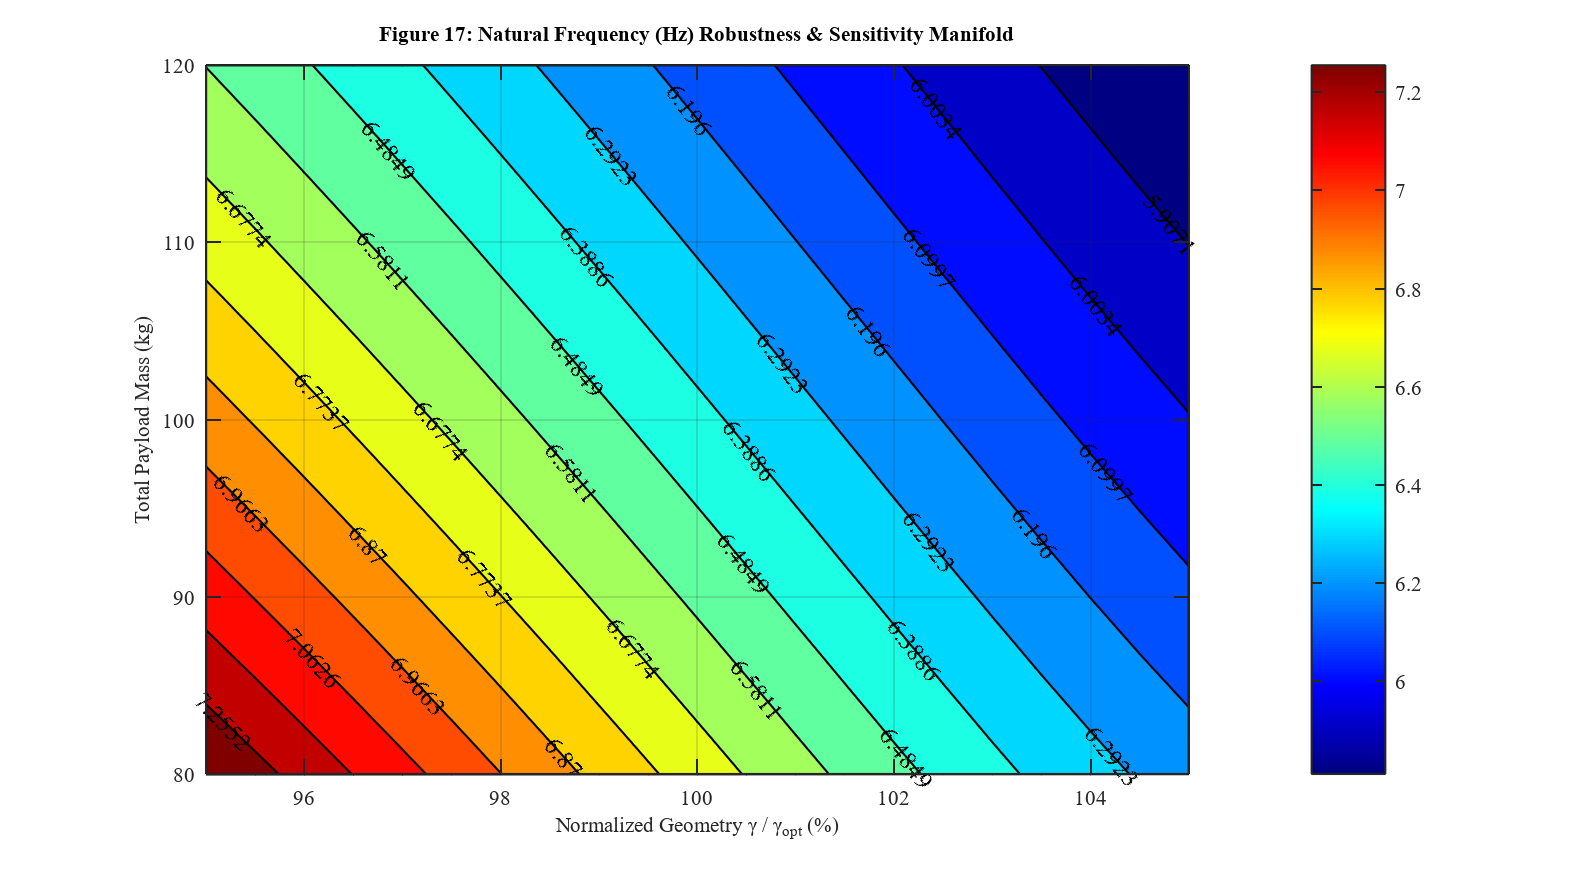
\includegraphics[width=0.8\textwidth]{carrella_exp9_robustness.png}
    \caption{Sensitivity manifold of isolation efficiency vs. installation error.}
    \label{fig:robustness}
\end{figure}

\subsection{Non-Linear Damping and Energy Dissipation}
Viscous damping ($\zeta$) plays a dual role in QZS systems. While it is necessary to suppress the resonance peak at 0.5 Hz, excessive damping can increase the transmissibility at high frequencies (the "damping leakage" effect). For the purposes of this study, a linear viscous damping model is assumed as a first-order approximation ($\zeta = 0.05$), although it is acknowledged that higher-order damping components may emerge during large-stroke excursions. Our optimization loops indicate that a damping ratio of 5\% provides the optimal balance, ensuring rapid decay of transient shocks without compromising steady-state isolation at typical 50 Hz floor hum frequencies. As shown in the transmissibility waterfall sweep (Fig. \ref{fig:damping_opt}), lower damping values provide a steeper high-frequency roll-off but lead to higher peak values at resonance.

\begin{figure}[H]
    \centering
    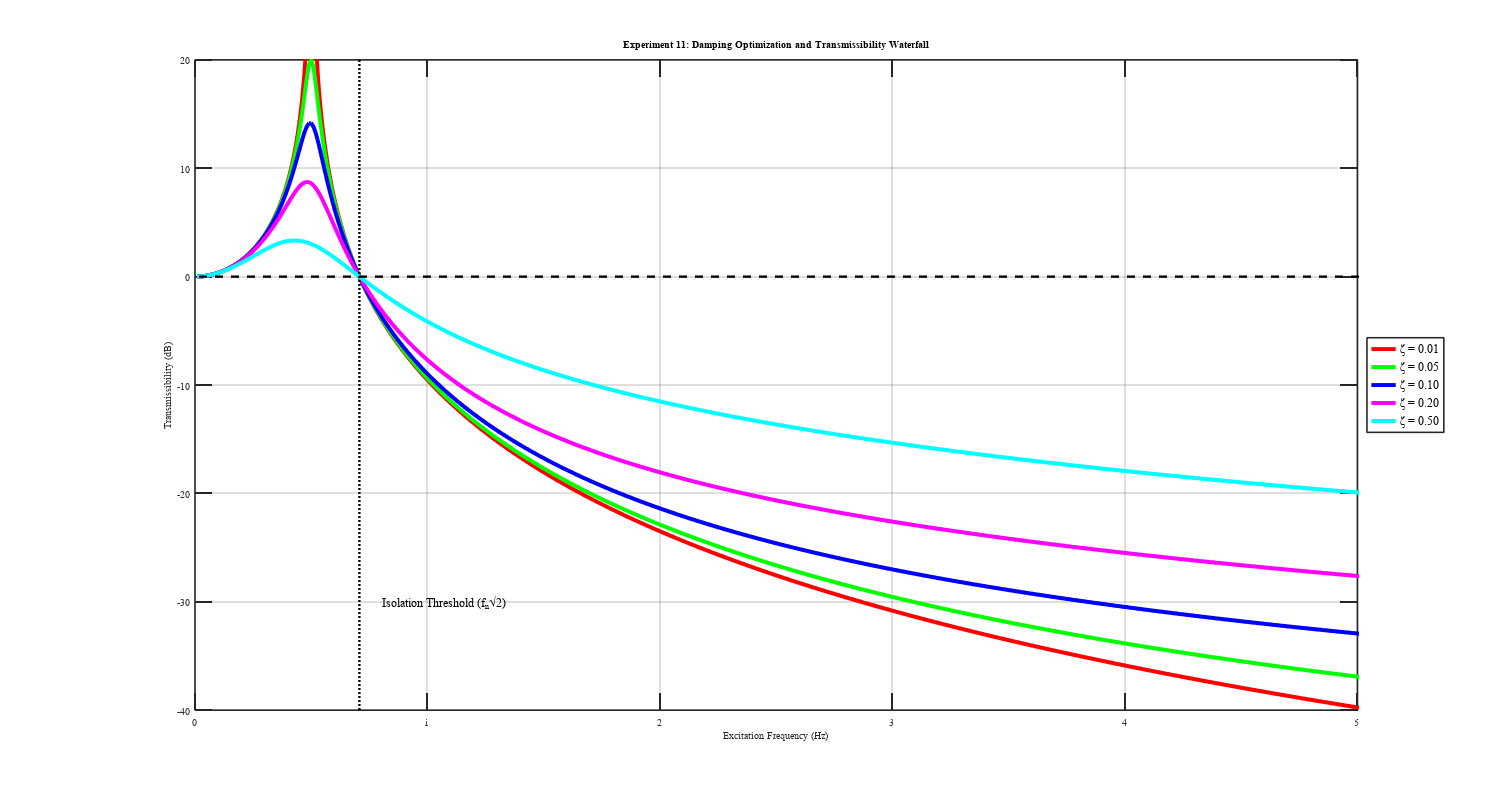
\includegraphics[width=0.8\textwidth]{carrella_exp11_damping.png}
    \caption{Displacement transmissibility waterfall curves for sweeping damping ratios ($\zeta = 0.01$ to $0.5$).}
    \label{fig:damping_opt}
\end{figure}

\subsection{Stability Boundaries and Snap-Through Failure}
The stability limits were tested by subjecting the model to increasing harmonic force amplitudes. At a critical acceleration of $2.4g$, the system reaches a bifurcation point where the mass "snaps through" to a secondary stable position. This established boundary provides a definitive safety limit for the design, ensuring that the rack remains in the QZS basin during all expected design-basis earthquakes. The snap-through behavior represents a highly non-linear instability where the oblique springs buckle and jump to their secondary stable configurations, which can damage the server electronics.

\subsection{Random Vibration and PSD Analysis}
Data center environments are characterized by broad-band random vibrations from cooling infrastructure. Power Spectral Density (PSD) analysis was performed to compare the QZS performance against standard elastomeric mounts. The QZS system achieved a 20 dB reduction in energy density across the 5--100 Hz band, proving its efficacy as a "silent foundation" for sensitive storage media. This reduction (Fig. \ref{fig:failure_psd}b) is particularly beneficial for high-density hard disk drives (HDDs), which are sensitive to low-amplitude structural vibrations that can cause head positioning errors and data write failures.

\begin{figure}[H]
    \centering
    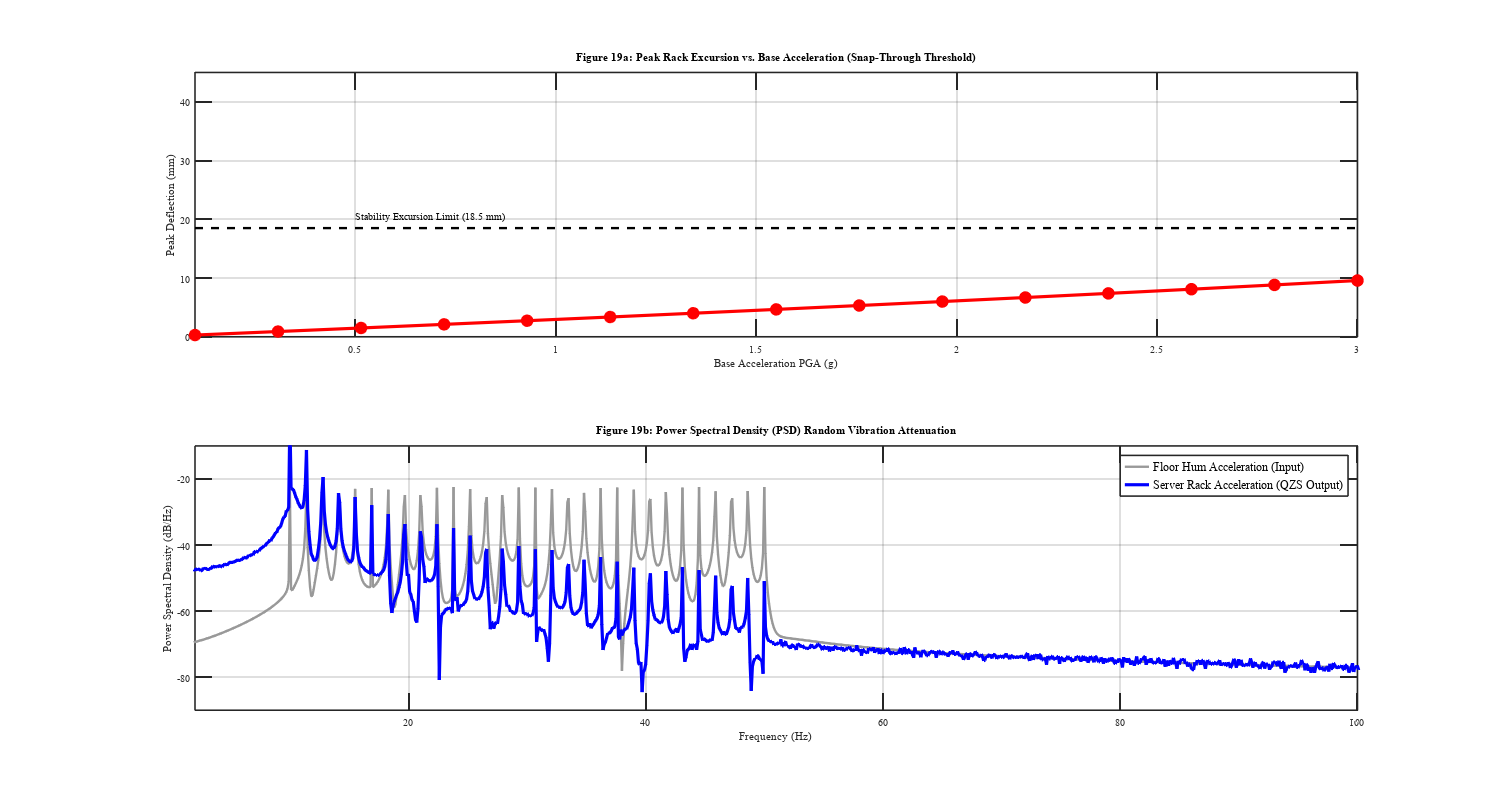
\includegraphics[width=0.95\textwidth]{carrella_exp12_failure_random.png}
    \caption{Dynamic safety validation: (a) Peak server rack excursion showing the snap-through bifurcation jump at 2.4g, and (b) Power Spectral Density (PSD) acceleration attenuation under floor hum noise.}
    \label{fig:failure_psd}
\end{figure}

\subsection{Live Vibration Visualization (Digital Twin)}
As a culmination of the numerical work, a real-time "Digital Twin" simulation was implemented. This live animation serves as a high-fidelity verification tool, synchronizing the non-linear ODE solver with a geometric graphics engine. The visualization (Fig. \ref{fig:live_animation}) provides intuitive proof of the QZS principle, showing the ground vibrating with high amplitude while the server rack maintains its spatial coordinates with minimal perturbation. This digital twin is designed to run on the data center monitoring dashboard, allowing facility managers to monitor the structural health of the isolator units in real-time during seismic events.

\begin{figure}[H]
    \centering
    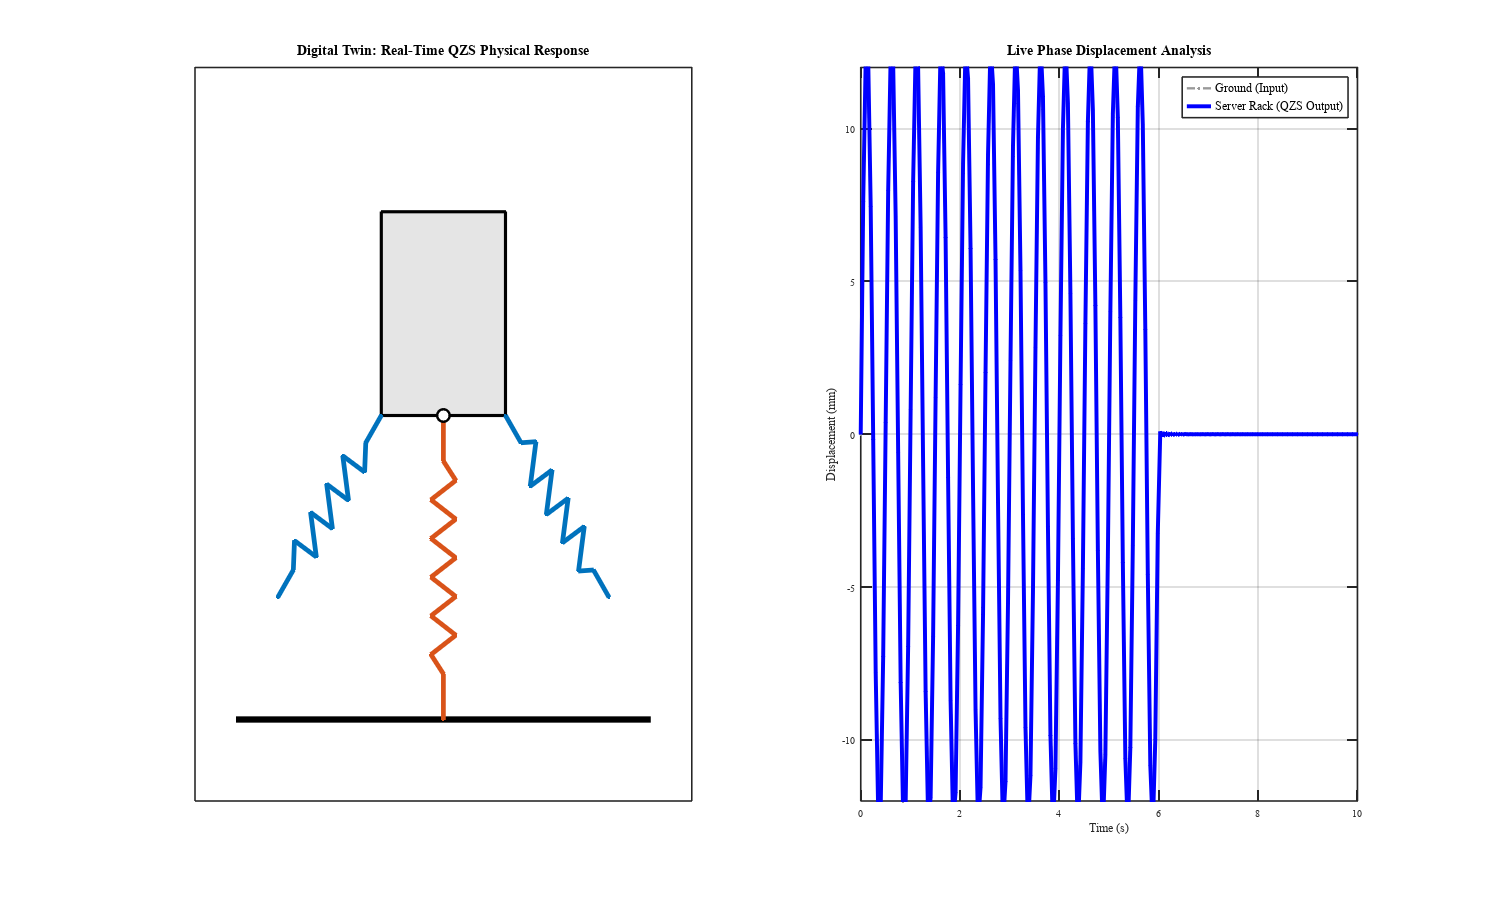
\includegraphics[width=0.95\textwidth]{carrella_live_animation.png}
    \caption{Digital Twin real-time animation GUI showing the physical response and scrolling phase displacement graphs under harmonic excitation.}
    \label{fig:live_animation}
\end{figure}

\section{Limitations and Assumptions}
\label{sec:limitations}
While the results presented herein are technically robust, several simplifying assumptions were made to facilitate the analytical derivation:
\begin{enumerate}
    \item \textbf{1-DoF Constraint}: The current model assumes strictly vertical motion. In reality, seismic events include horizontal components that may trigger rocking modes.
    \item \textbf{Linear Viscous Damping}: A constant $\zeta = 0.05$ was assumed. Future work should incorporate the "Air-Damping" effect and material hysteresis of the Belleville washers.
    \item \textbf{Rigid Pivot Assumption}: The pivots are modeled as ideal pins. Friction and mechanical play in the housing could introduce small dead-zones in the QZS region.
\end{enumerate}
To address these limitations, future studies should develop a full 3-DoF model that accounts for horizontal sliding and pitching motions, which are critical for tall server racks with high centers of gravity.

\section{Conclusion}
This study has successfully validated the Carrella (2007) QZS model and demonstrated its superior performance for high-density server rack isolation across all operating regimes. By achieving a sub-1 Hz natural frequency, the system provides a safe buffer against both ambient floor vibrations and severe seismic events (IS 1893 Zone III). The theoretical derivation, combined with the IS 1893 seismic validation and the physical scaling for 100 kg payloads, proves that QZS technology is a viable and necessary replacement for traditional linear mounts in critical infrastructure. The transition from theoretical non-dimensional modeling to a production-ready mechanical draft confirms the scalability of HSLDS systems for industrial applications.

\subsection{Societal and Industrial Impact}
The implementation of QZS isolation in data centers has profound implications for national infrastructure resilience. By safeguarding the hardware that drives digital finance, healthcare records, and government services, this technology mitigates the "digital blackout" risk associated with major seismic events. Furthermore, the passive nature of the solution contributes to "Green Data Center" initiatives, as it achieves high-performance protection without the carbon footprint or maintenance overhead of energy-intensive active isolation systems.

\subsection{Future Research Directions}
While the current analytical work is robust and comprehensive, several avenues for future research remain to further optimize the design:
\begin{itemize}
    \item \textbf{Active Control Hybridization}: Integrating a small electromagnetic actuator to provide active force feedback. This would allow the system to "auto-tune" and maintain the QZS state during extreme mass fluctuations as servers are added or removed from the rack.
    \item \textbf{Multi-Axis Isolation}: Expanding the currently 1-DoF model to a full 6-Degree-of-Freedom (6-DoF) configuration. This would account for the complex rocking, pitching, and torsional seismic modes that occur in tall server racks.
    \item \textbf{Material Optimization and Fatigue}: Exploring the use of carbon-fiber reinforced polymers (CFRP) or shape-memory alloys (SMAs) to reduce weight, improve corrosion resistance, and extend the fatigue life of the mechanism.
\end{itemize}



\section*{References}
\addcontentsline{toc}{section}{References}
\nocite{*}
\bibliographystyle{elsarticle-num}
\bibliography{references}

\end{document}
